%%%
%
% $Autor: Wings $
% $Datum: 2021-05-14 $
% $Pfad: ArduinoIDE2 $
% $Dateiname: 
% $Version: 4620 $
%
% !TeX spellcheck = de_DE/GB
% !TeX program = pdflatex
% !BIB program = biber/bibtex
% !TeX encoding = utf8
%
%%%



\chapter{Arduino IDE 2.3.x}\label{ArduinoIDE2}



In this chapter we will be going through the description of the Arduino IDE and describe the features of it and what are all the options present in the IDE and how can we use it. Further we will be describing about the installation procedure of the Arduino IDE and how to get started with it.


\section{Arduino IDE Description}\label{ArduinoIDE}

It is an open source official Arduino software which used for editing, uploading and compiling codes in to the Arduino module. It is a cross-platform software which is available for Operating Systems like Windows, Linux, macOS. It runs on Java platform and supports a range of Arduino modules. It supports C and C++ languages. The microcontrollers present on the Arduino boards are programmed which accepts the information in the form of code. The program written in the IDE is called a sketch which will generate a Hex file which is then transferred and uploaded in the controller.
The IDE environment is made up of two parts: an editor and a compiler. The editor is used to write the required code, while the compiler is used to compile and upload the code to the Arduino Module.\cite{Fezari:2018}
The Menu bar has options such as File in which there are many options including Opening a new file or existing, Examples-in which we can find sketches for different applications like Blink, Fade etc. There is an error console at the bottom of the screen for displaying errors.

The 6 buttons are present on top of the screen are as follows:

\begin{figure}[H]\centering
    
\includegraphics[width=8cm]{Arduino/ArdiunoIDE2/MenuButton}
    
    \caption{\textbf{Menu Button.}}
    \label{fig::Menu Button}		
\end{figure}


\begin{itemize}
    \item	The check mark is used to verify your code. Click this once you have written your code.
    \item	The arrow uploads your code to the Arduino to run.
    \item	The dotted paper will create a new file.
    \item	The upward arrow is used to open an existing Arduino project.
    \item	The downward arrow is used to save the current file.
    \item	The far right button is a serial monitor, which is useful for sending data from the Arduino to the PC for debugging purposes.
\end{itemize}




\section{Installation on Windows}

\subsection{Download}
You can easily download the editor from the Arduino Software page. ~\ref{Download}
\begin{figure}
    \begin{center}
        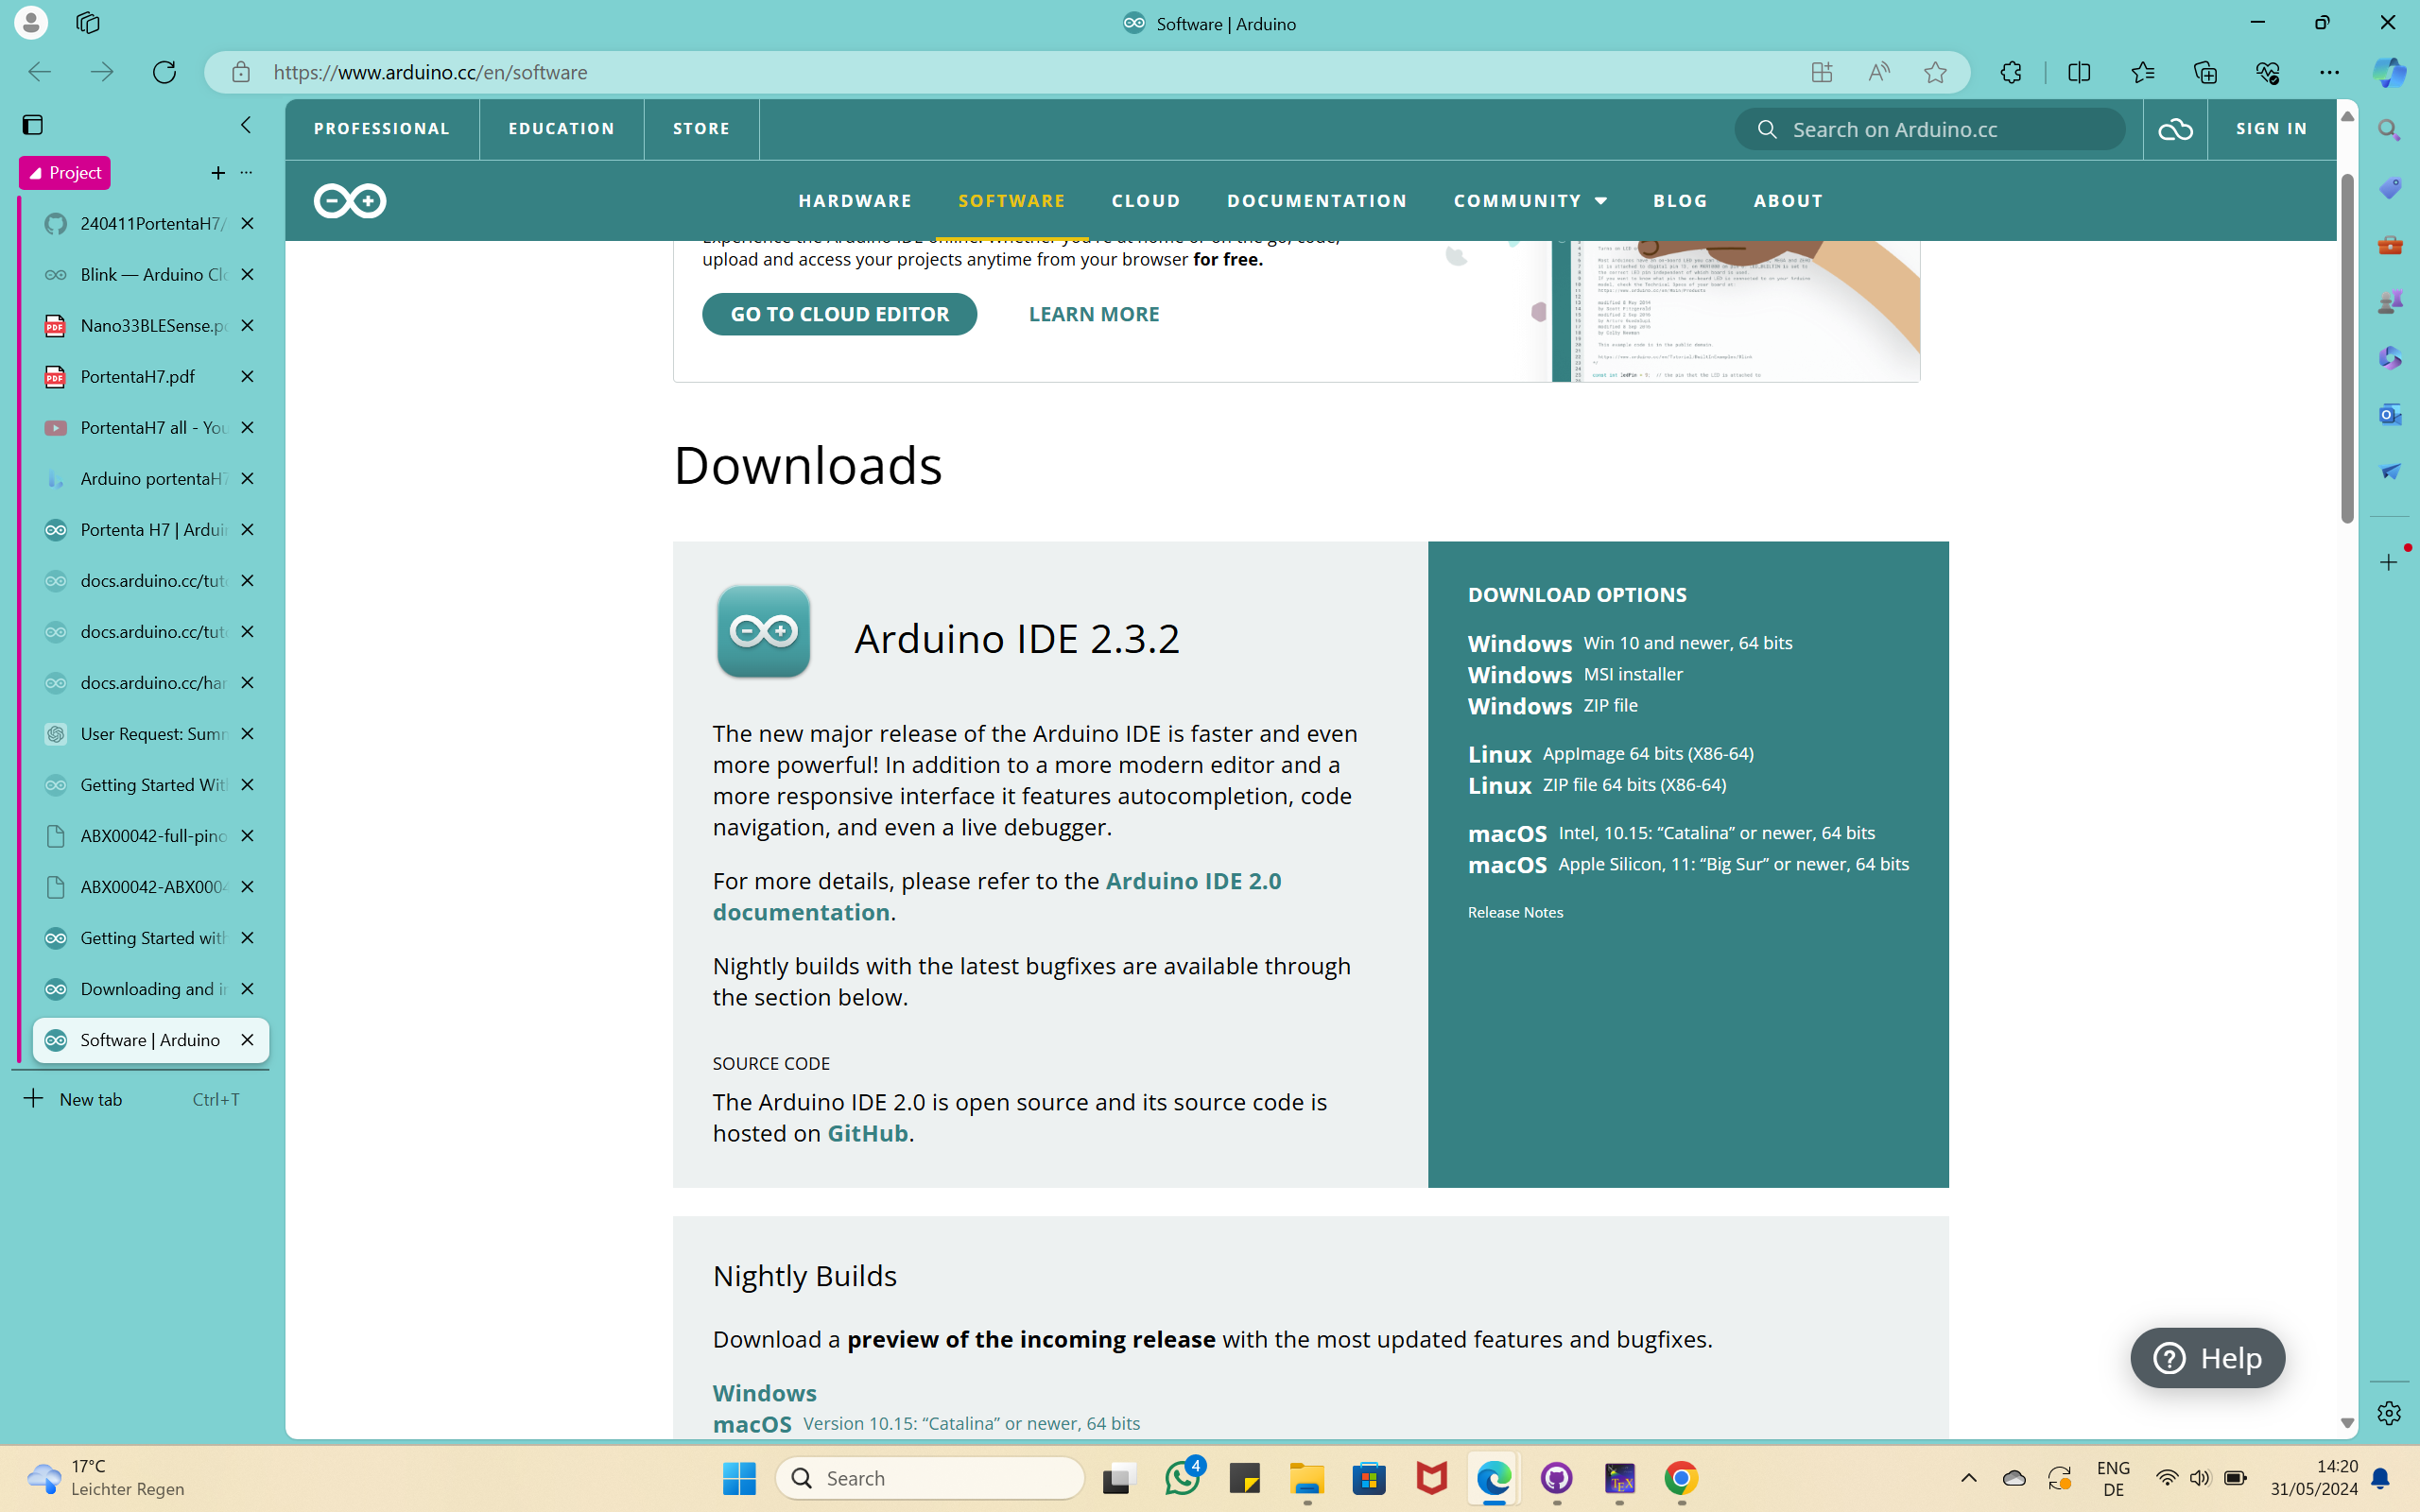
\includegraphics[width=0.7\linewidth]{Arduino/ArdiunoIDE2/DownloadArduinofile.png}
        \caption{Arduino File}
        \label{Download}
    \end{center}
\end{figure}

\subsection{Installation}
To install the Arduino IDE 2 on a Windows computer, simply run the file downloaded from the software page.~\ref{downloading-and-installing-img01} ~\ref{downloading-and-installing-img02}
\begin{figure}
    \begin{center}
        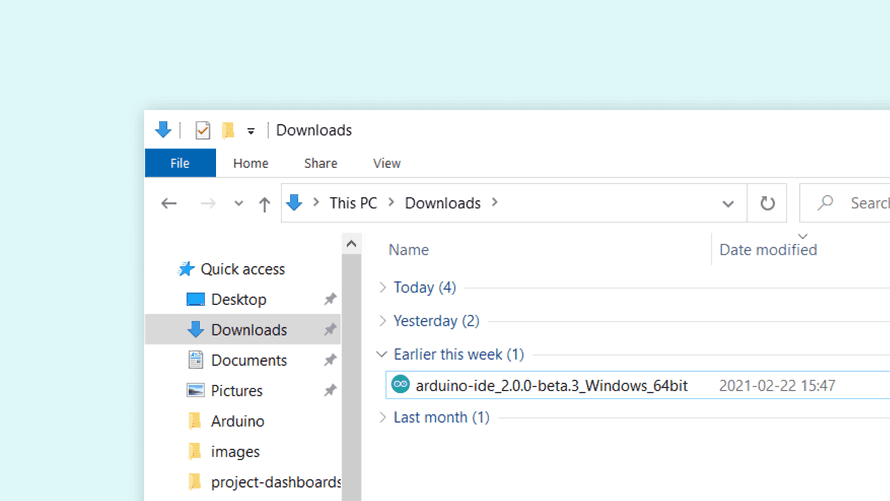
\includegraphics[width=0.7\linewidth]{Arduino/ArdiunoIDE2/downloading-and-installing-img01.png}
        \caption{Running the installation file}
        \label{downloading-and-installing-img01}
    \end{center}
\end{figure}


\begin{figure}
    \begin{center}
        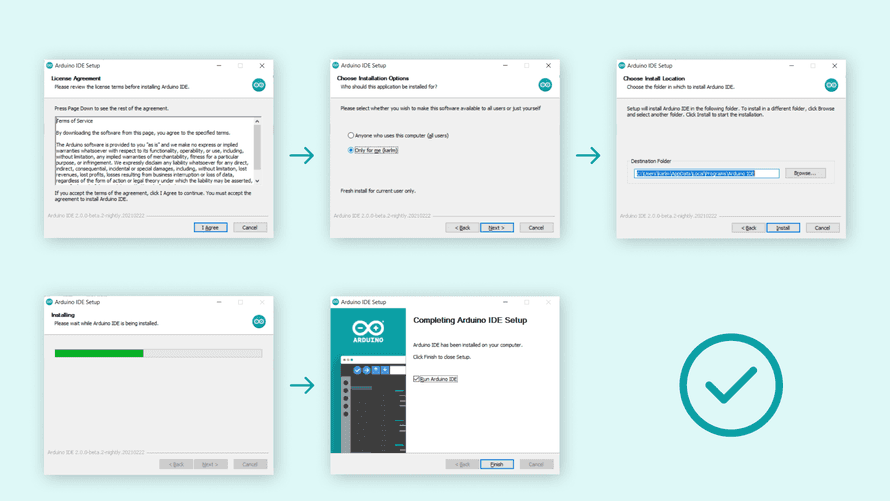
\includegraphics[width=0.7\linewidth]{Arduino/ArdiunoIDE2/downloading-and-installing-img02.png}
        \caption{Steps for Installation}
        \label{downloading-and-installing-img02}
    \end{center}
\end{figure}

\section{Overview}
The Arduino IDE 2 features a new sidebar, making the most commonly used tools more accessible. ~\ref{ide-2-overview} \cite{arduinodescription:2024}

\begin{itemize}
    \item \textbf{Verify / Upload}- compile and upload your code to your Arduino Board.
    \item \textbf{Select Board and Port}- detected Arduino boards automatically show up here, along with the port number.
    \item \textbf{Sketchbook}- here you will find all of your sketches locally stored on your computer. Additionally, you can sync with the Arduino Cloud, and also obtain your sketches from the online environment.
    \item \textbf{Boards Manager}- browse through Arduino and third party packages that can be installed. For example, using a MKR WiFi 1010 board requires the Arduino SAMD Boards package installed.
    \item \textbf{Library Manager}- browse through thousands of Arduino libraries, made by Arduino and its community.
    \item \textbf{Debugger}- test and debug programs in real time.
    \item \textbf{Search}- search for keywords in your code.
    \item \textbf{Open Serial Monitor}- opens the Serial Monitor tool, as a new tab in the console.
\end{itemize}

\begin{figure}
    \begin{center}
        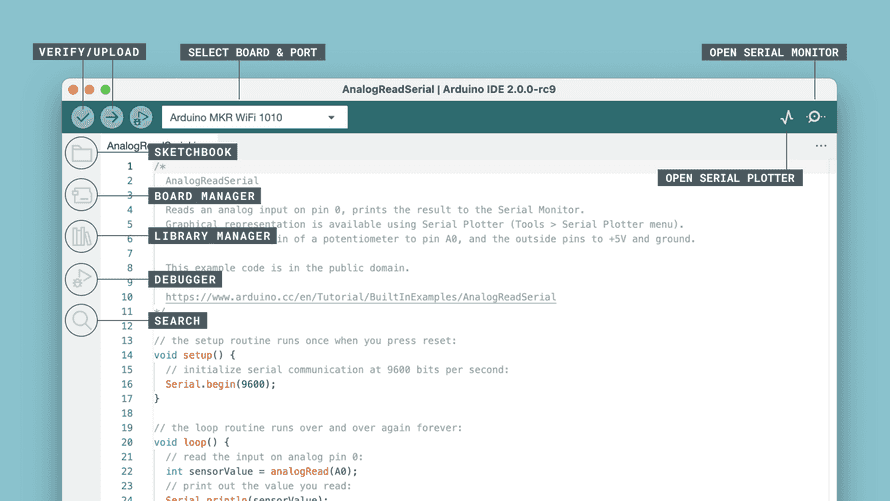
\includegraphics[width=0.7\linewidth]{Arduino/ArdiunoIDE2/ide-2-overview.png}
        \caption{Overview}
        \label{ide-2-overview}
    \end{center}
\end{figure}

\section{Features}
The Arduino IDE 2 is a versatile editor with many features. You can install libraries directly, sync your sketches with Arduino Cloud, debug your sketches and much more. In this section, some of the core features are listed, along with a link to a more detailed article. 

\subsection{Sketchbook}
Your sketchbook is where your code files are stored. Arduino sketches are saved as .ino files, and must be stored in a folder of the exact name. For example, a sketch named my sketch.ino must be stored in a folder named my sketch. ~\ref{local-sketchbook}

Typically, your sketches are saved in a folder named Arduino in your Documents folder.

To access your sketchbook, click on the folder icon located in the sidebar.
\begin{figure}
    \begin{center}
        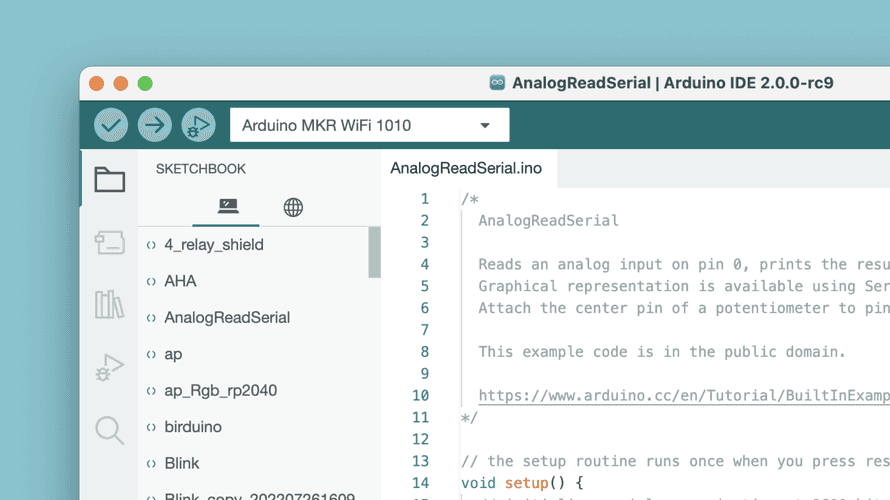
\includegraphics[width=0.7\linewidth]{Arduino/ArdiunoIDE2/local-sketchbook.png}
        \caption{Sketchbook}
        \label{local-sketchbook}
    \end{center}
\end{figure}

\subsection{Boards Manager}
With the Boards Manager, you can browse and install board packages. A board package contains the "instructions" for compiling your code to the boards that are included in the board package. ~\ref{board-manager}

There are several Arduino board packages available, such as avr, samd, megaavr and more.
\begin{figure}
    \begin{center}
        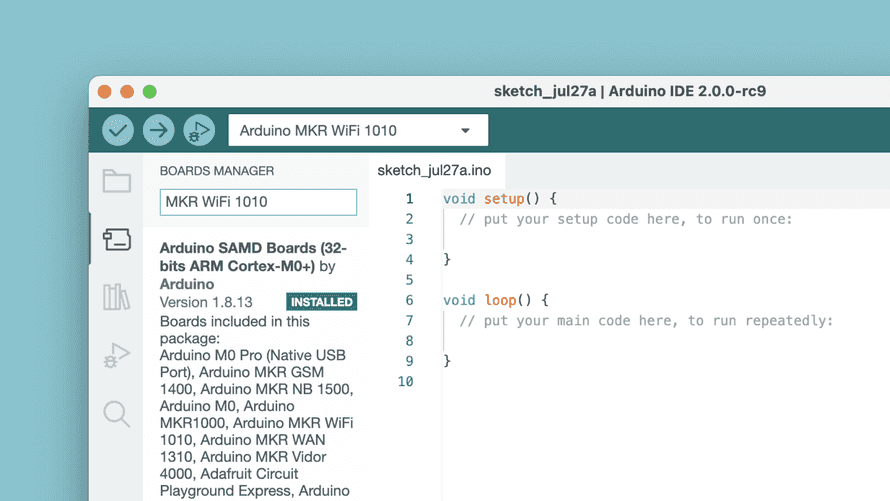
\includegraphics[width=0.7\linewidth]{Arduino/ArdiunoIDE2/board-manager.png}
        \caption{Board-Manager}
        \label{board-manager}
    \end{center}
\end{figure}

\subsection{Library Manager}
With the library manager you can browse and install thousands of libraries. Libraries are extensions of the Arduino API, and makes it easier to for example control a servo motor, read specific sensors, or use a Wi-Fi module. ~\ref{library-manager}

\begin{figure}
    \begin{center}
        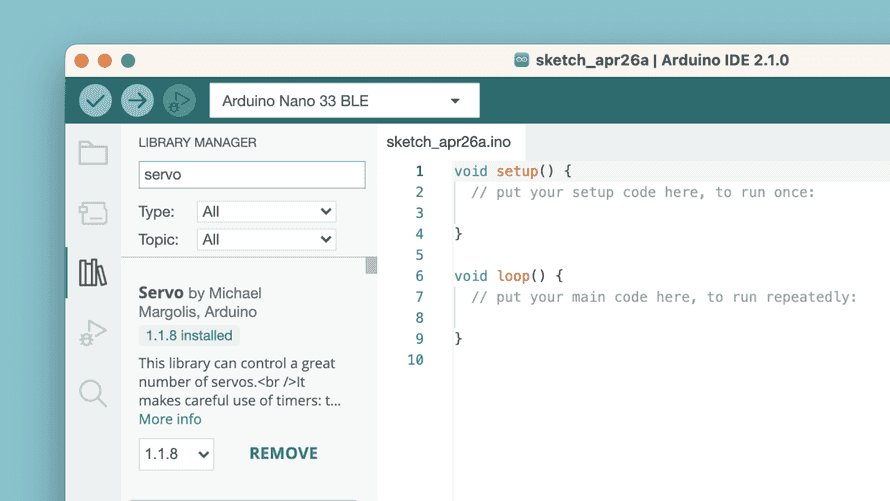
\includegraphics[width=0.7\linewidth]{Arduino/ArdiunoIDE2/library-manager.png}
        \caption{library-manager}
        \label{library-manager}
    \end{center}
\end{figure}

\subsection{Serial Monitor}
The Serial Monitor is a tool that allows you to view data streaming from your board, via for example the Serial.print() command.

Historically, this tool has been located in a separate window, but is now integrated with the editor. This makes it easy to have multiple instances running at the same time on your computer. ~\ref{serial-monitor}

\begin{figure}
    \begin{center}
        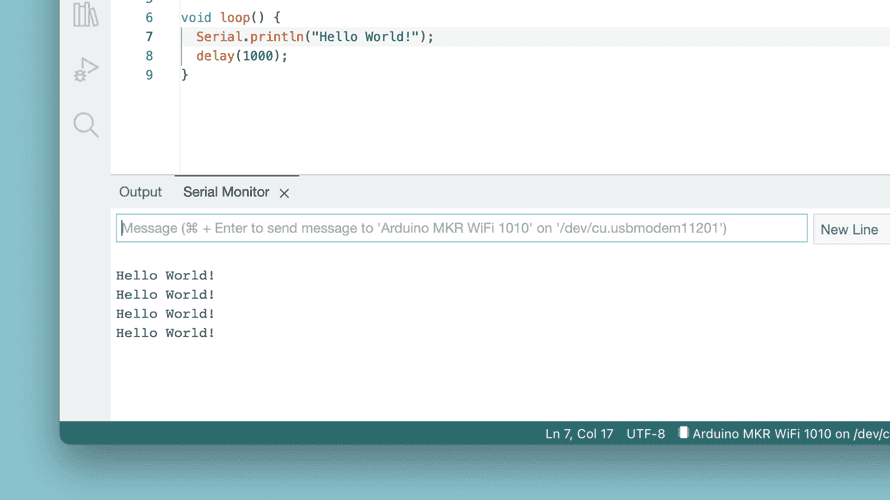
\includegraphics[width=0.7\linewidth]{Arduino/ArdiunoIDE2/serial-monitor.png}
        \caption{serial-monitor}
        \label{serial-monitor}
    \end{center}
\end{figure}

\subsection{Serial Plotter}
The Serial Plotter tool is great for visualizing data using graphs, and to monitor for example peaks in voltage.

You can monitor several variables simultaneously, with options to enable only certain types. 

\section{Examples}
An important part of the Arduino Documentation are the example sketches that come bundled with libraries. They will show examples of the functions used in practice, illustrating the intended use and features of a library.

Libraries that come bundled as a part of a boards package may also include libraries, and those libraries often include example sketches.

To open the example sketches bundled in either the libraries you have installed manually or that come bundled in board packages, navigate to File > Examples and find the library you're searching for in the list that appears. ~\ref{examplesketches}

\begin{figure}
    \begin{center}
        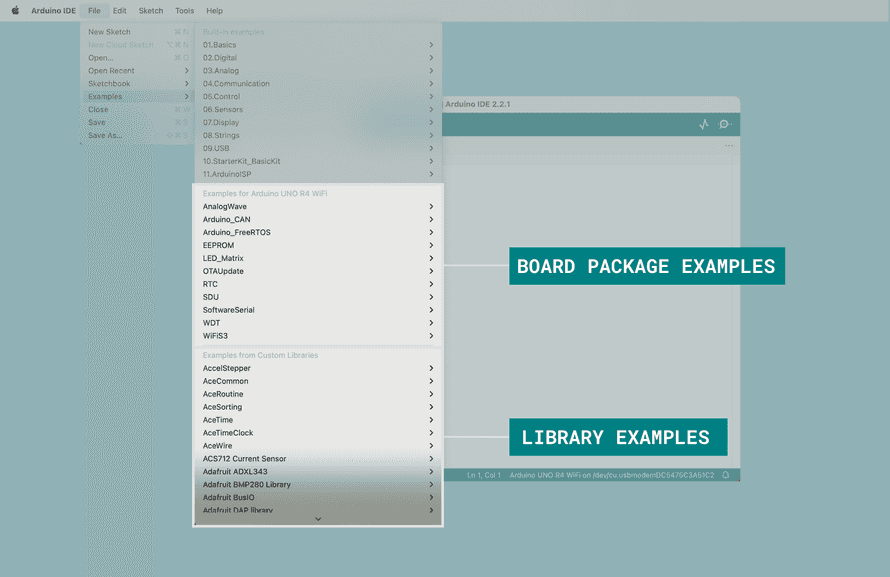
\includegraphics[width=0.7\linewidth]{Arduino/ArdiunoIDE2/examplesketches.png}
        \caption{Example}
        \label{examplesketches}
    \end{center}
\end{figure}

In the image above, you can see what the examples list looks like when a UNO R4 WiFi board is connected to your computer.

From here, you can for example navigate to File - Examples - LED Matrix - MatrixIntro and upload the sketch to your board to show the Tetris animation that came pre-loaded on your UNO R4 WiFi when you first took it out of its box.

\section{Debugging}

The debugger tool is used to test and debug programs, hence the name. It can be used to navigate through a program's execution in a controlled manner. ~\ref{Debug}

\begin{figure}
    \begin{center}
        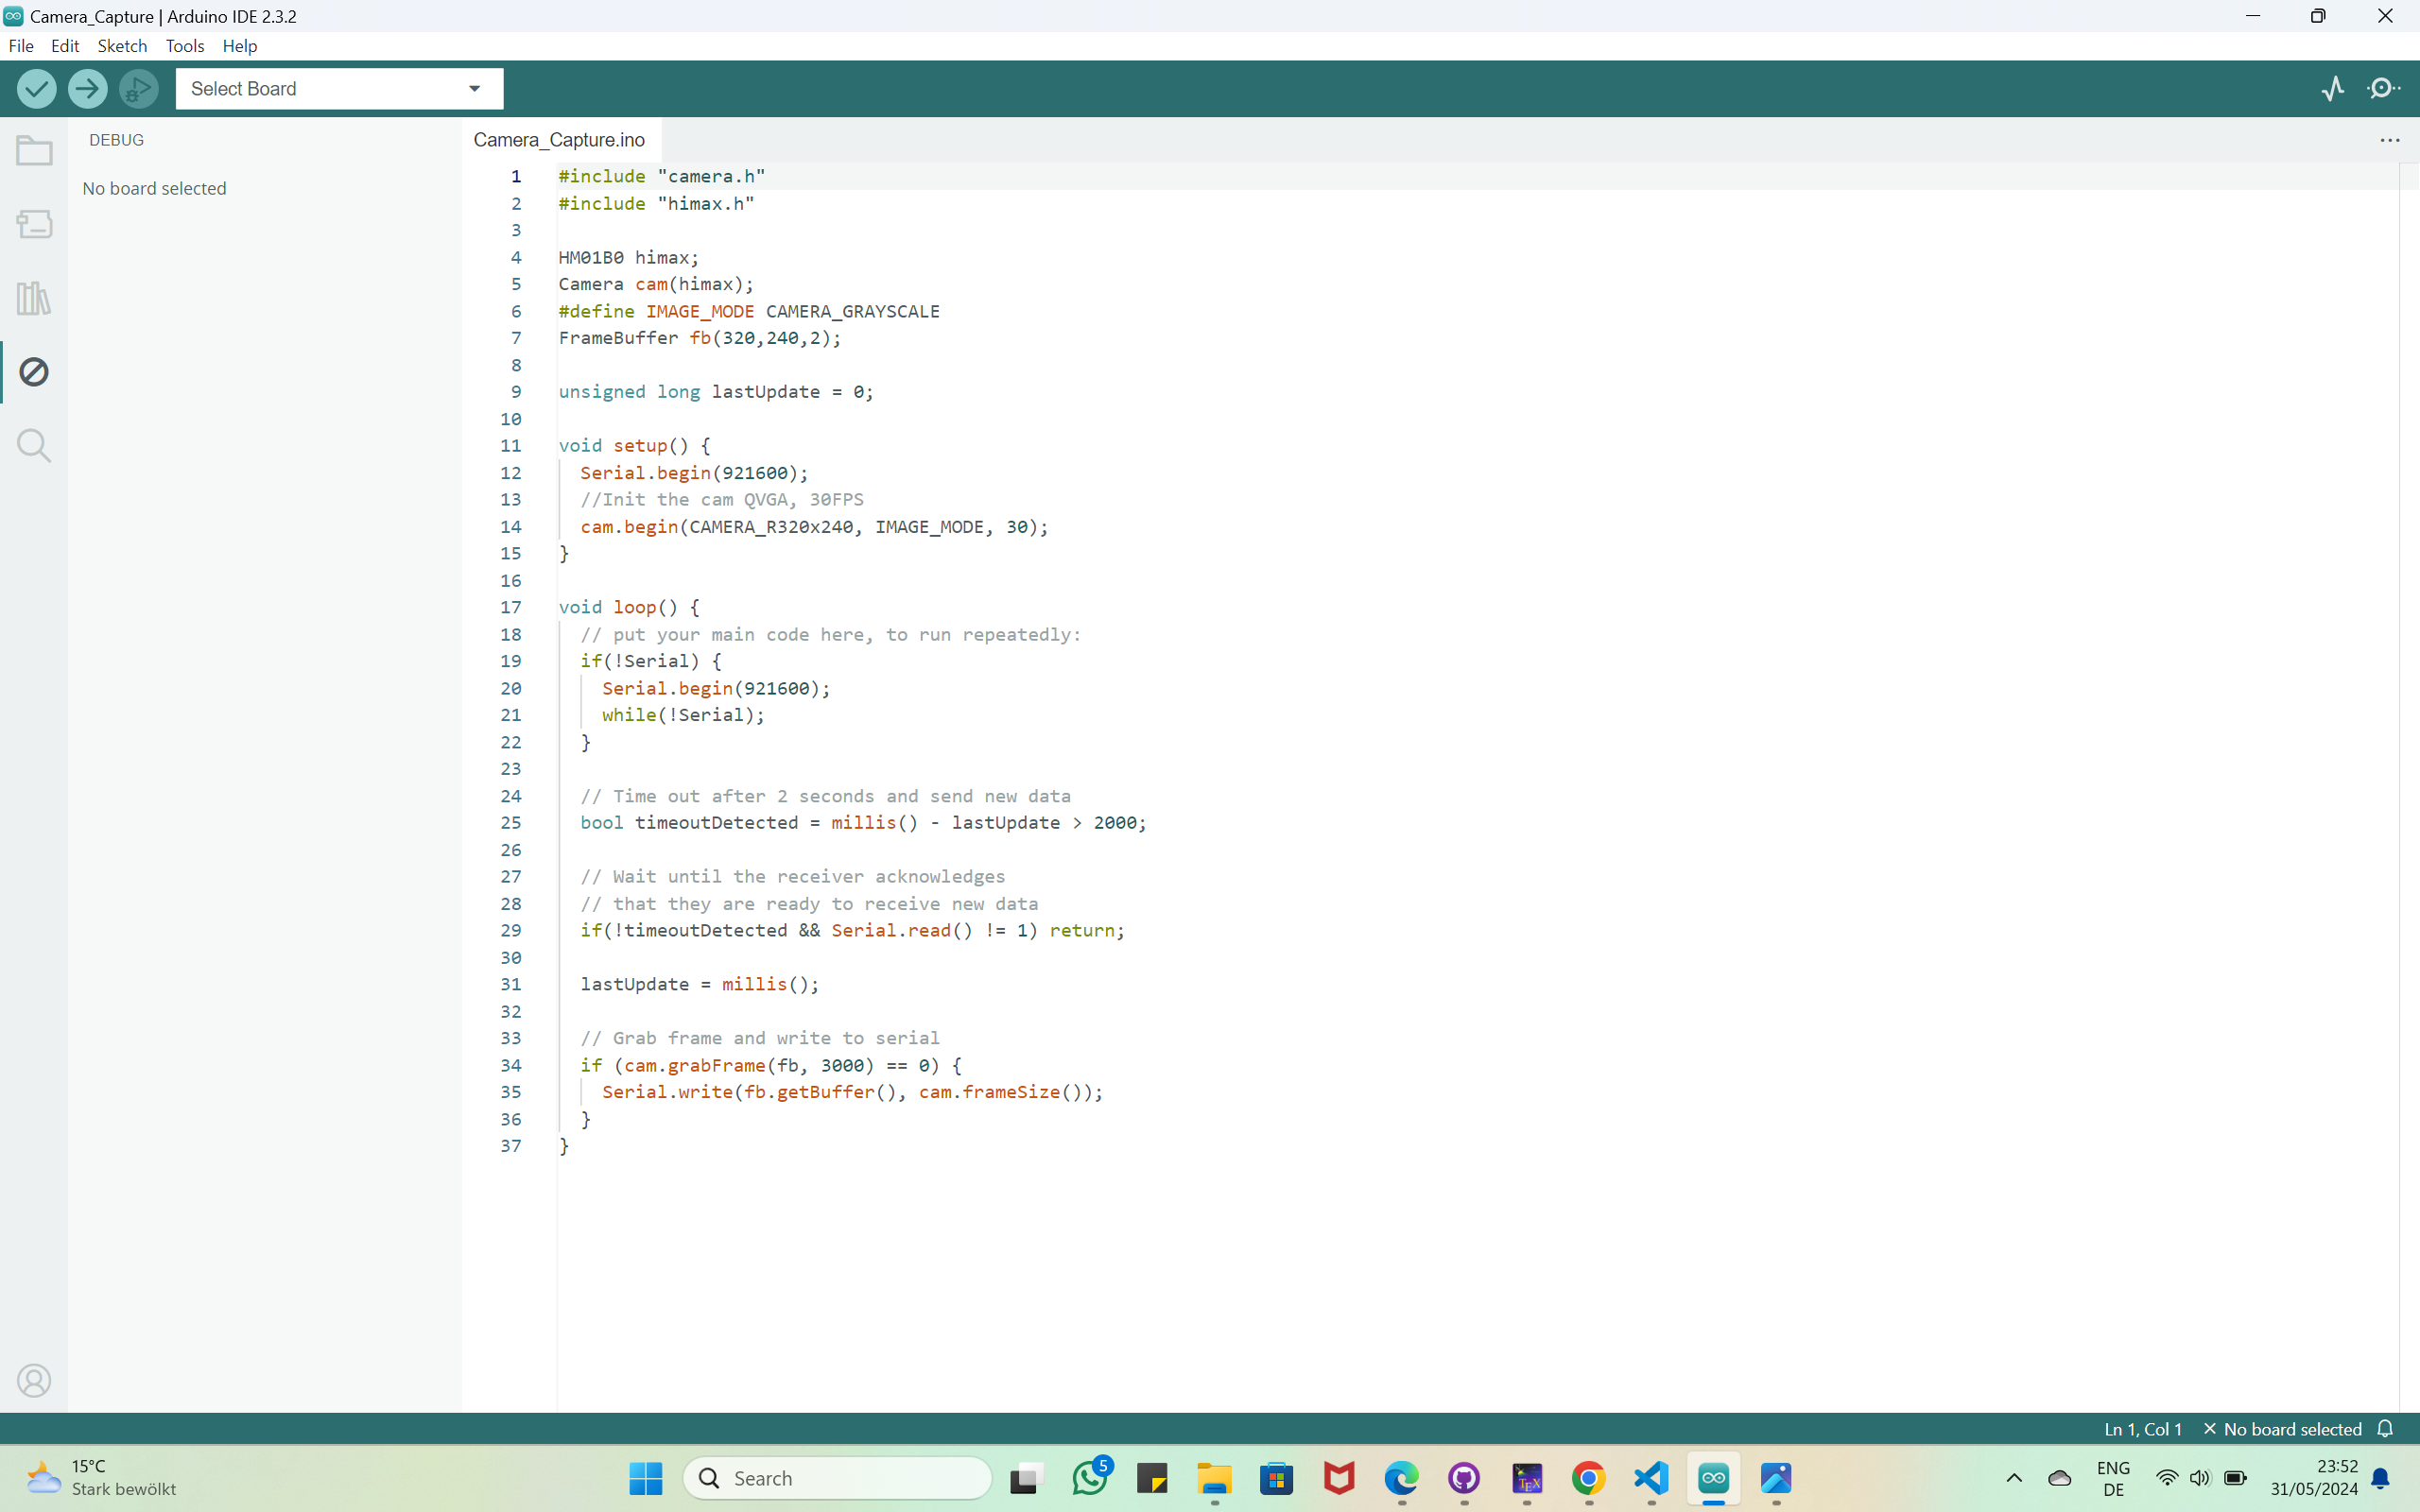
\includegraphics[width=0.7\linewidth]{Arduino/ArdiunoIDE2/Debug.png}
        \caption{Debugging}
        \label{Debug}
    \end{center}
\end{figure}

\section{Autocompletion}
Autocompletion is a must-have for code editors, and the 2 version comes well equipped. When writing code, this is useful to understand more about the elements of the Arduino API.

Note that you always need to select your board for autocompletion to work. ~\ref{autocomplete}

\begin{figure}
    \begin{center}
        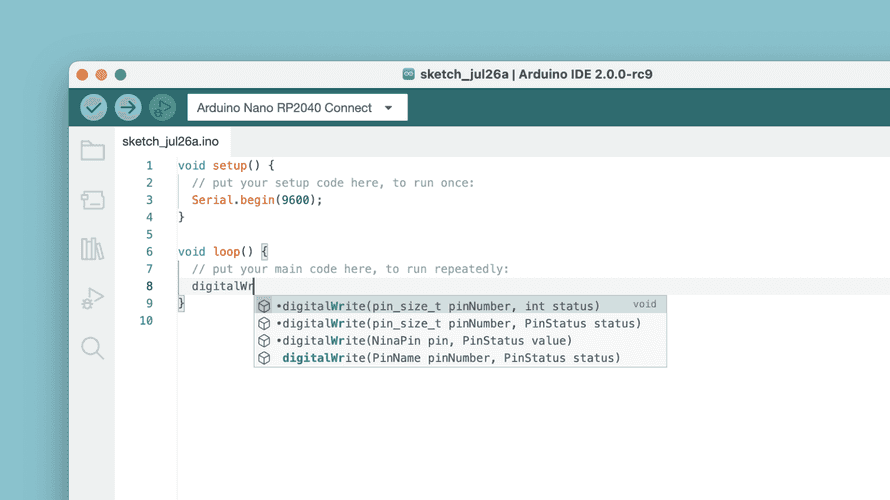
\includegraphics[width=0.7\linewidth]{Arduino/ArdiunoIDE2/autocomplete.png}
        \caption{autocomplete}
        \label{autocomplete}
    \end{center}
\end{figure}

\section{Conclusion}
In this guide, we have presented a series of features and more detailed articles to follow, so that you can enjoy each and every one of the features included in the IDE 2.


\section{Installation}

\subsection{Installation on Wondows}\label{Arduinoide}



Arduino Nano 33 BLE Sense uses the Arduino software integrated development environment (IDE) for programming, which is the most widely used and common (IDE) for all arduino boards that can be run online and offline. This is a open-source Arduino Software (IDE) makes it easy to write code and upload it to the board. There are various version of software which is supported for each operating system (OS) e.g: mac, linux, and windows. Arduino community also provide us to start coding online and save our sketches in the cloud, this online arduino editor is most up-to-date version of the IDE includes all libraries and also supports new Arduino boards. For getting access to these software packages go to the following link \url{https://www.arduino.cc/en/software}  and get more up to date inforamtion, because every single day there are some updates occurs which is available on the link mention above. These software can be used with any Arduino board, the most recent offline arduino IDE 1.8.15 can be seen in Figure,\ref{fig:Arduino Creat Agent Installation}. it is also supportive for all operating systems.
\Mynote{citations instead of links, why 1.8.15?}

\begin{figure}[H]\centering
    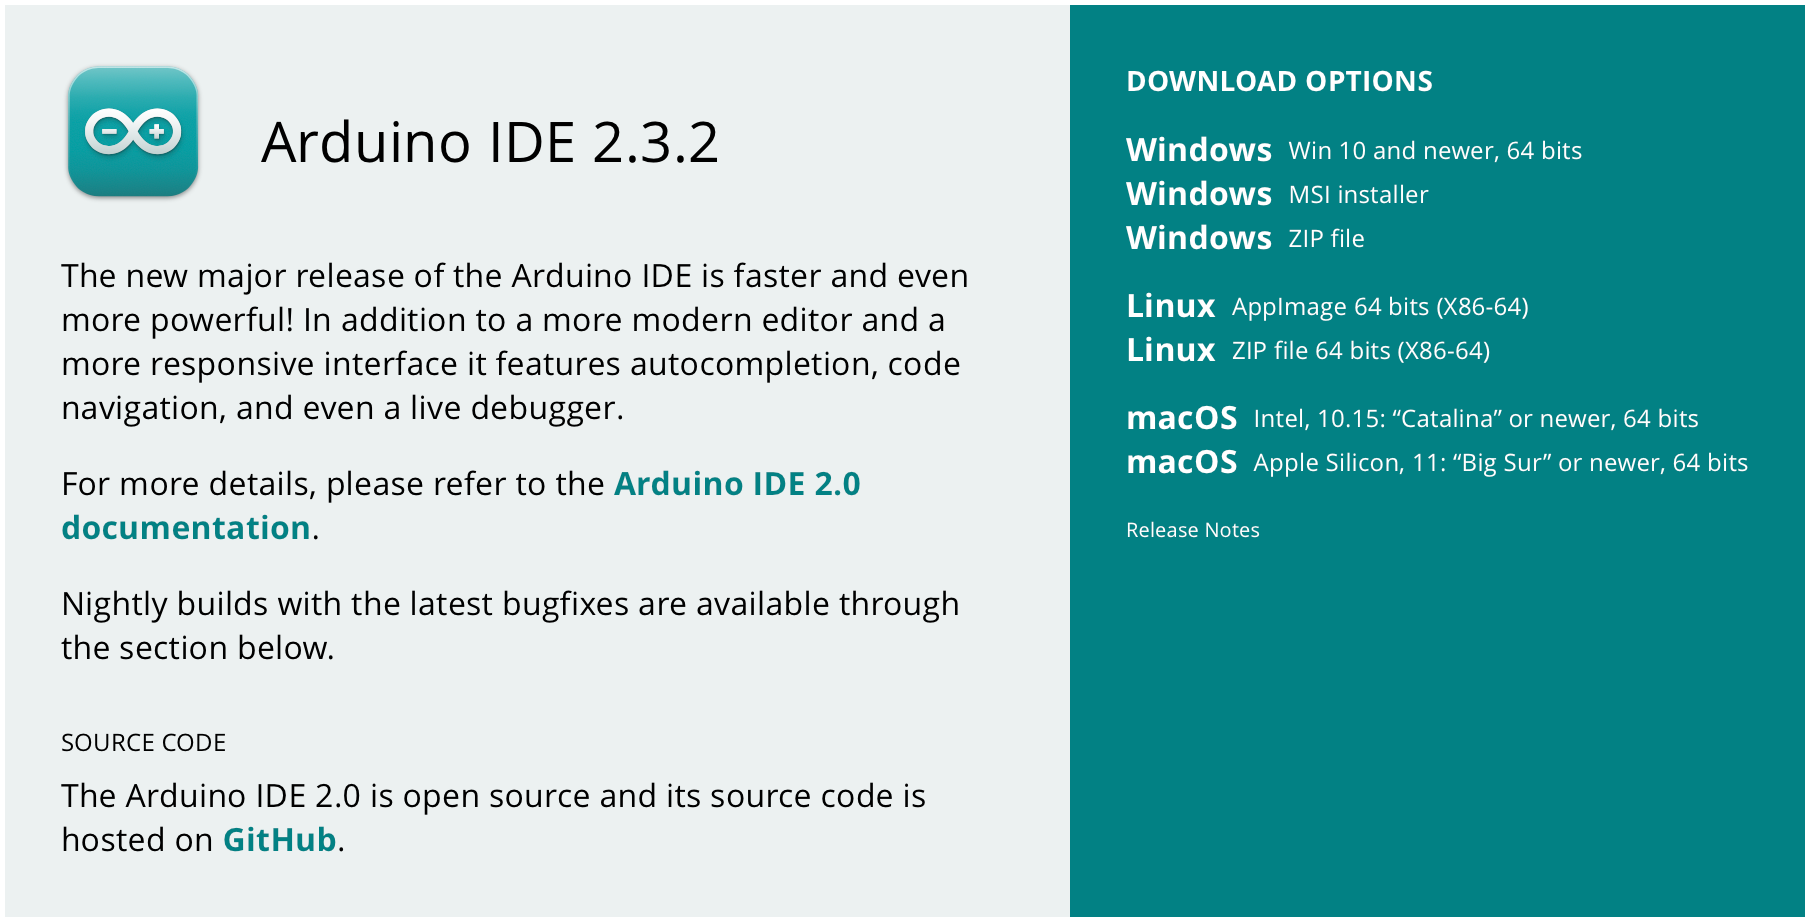
\includegraphics[width=8cm]{Arduino/ArdiunoIDE2/ArduinoIDECreateAgentInstallation.png}
    \caption{\textbf{Arduino IDE Creat Agent Installation.}}
    \label{fig:Arduino IDE Creat Agent Installation}		
\end{figure}

\begin{figure}[H]\centering
    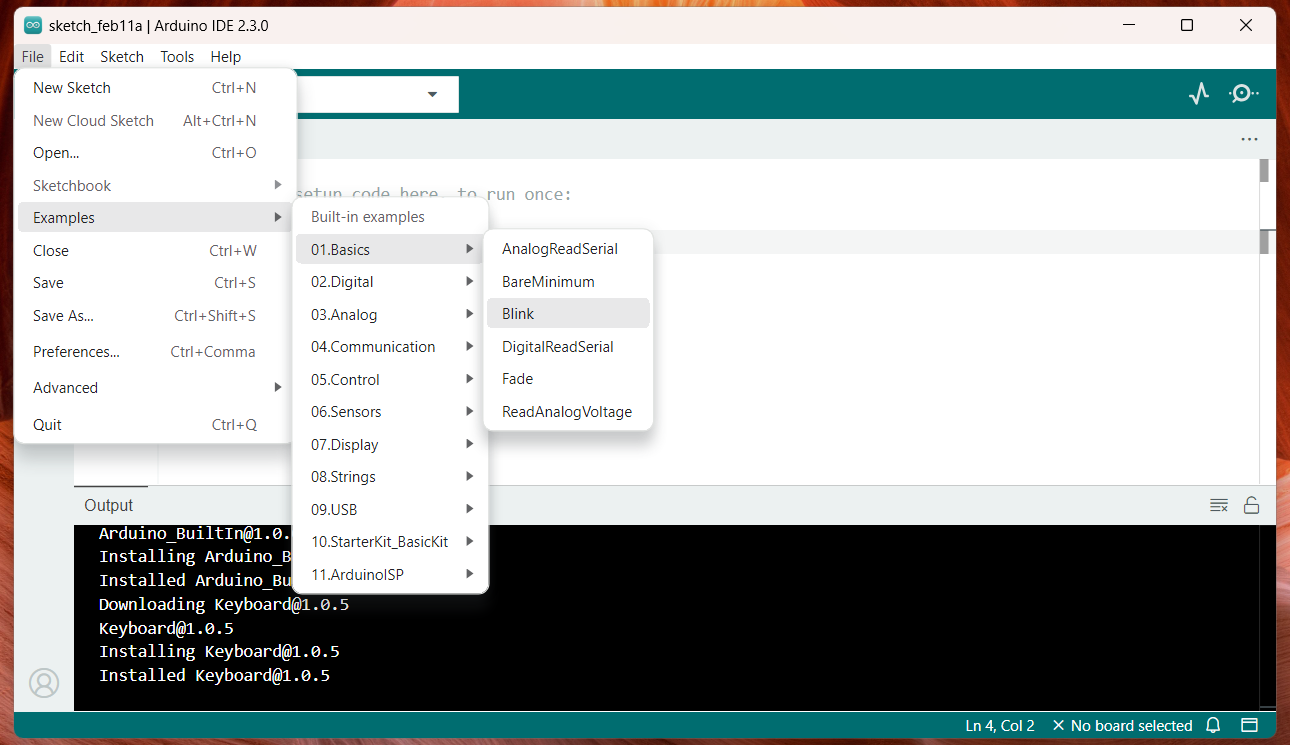
\includegraphics[width=8cm]{Arduino/ArdiunoIDE2/MenuBarOption}
    \caption{\textbf{Menu Bar Option.}}
    \label{fig::Menu Bar Option}		
\end{figure}

After the download is done, open the setup file and proceed to install.
Select all the components in the dialog box and click Next.

\begin{figure}[H]\centering
    \includegraphics[width=8cm]{Arduino/ArdiunoIDE2/ArduinoSetupInstallationOptions}
    \caption{\textbf{Arduino Setup Installation options.}}
    \label{fig:Arduino Setup Installation options}		
\end{figure}

Select the destination folder and click Install

\begin{figure}[H]\centering
    \includegraphics[width=8cm]{Arduino/ArdiunoIDE2/ArduinoSetupInstallationFolder}
    \caption{\textbf{Arduino Setup Installation Folder.}}
    \label{fig:Arduino Setup Installation Folder}		
\end{figure}

Once the installation is done, open the Arduino IDE and a default sketch appears on the screen as shows.

\begin{figure}[H]\centering
    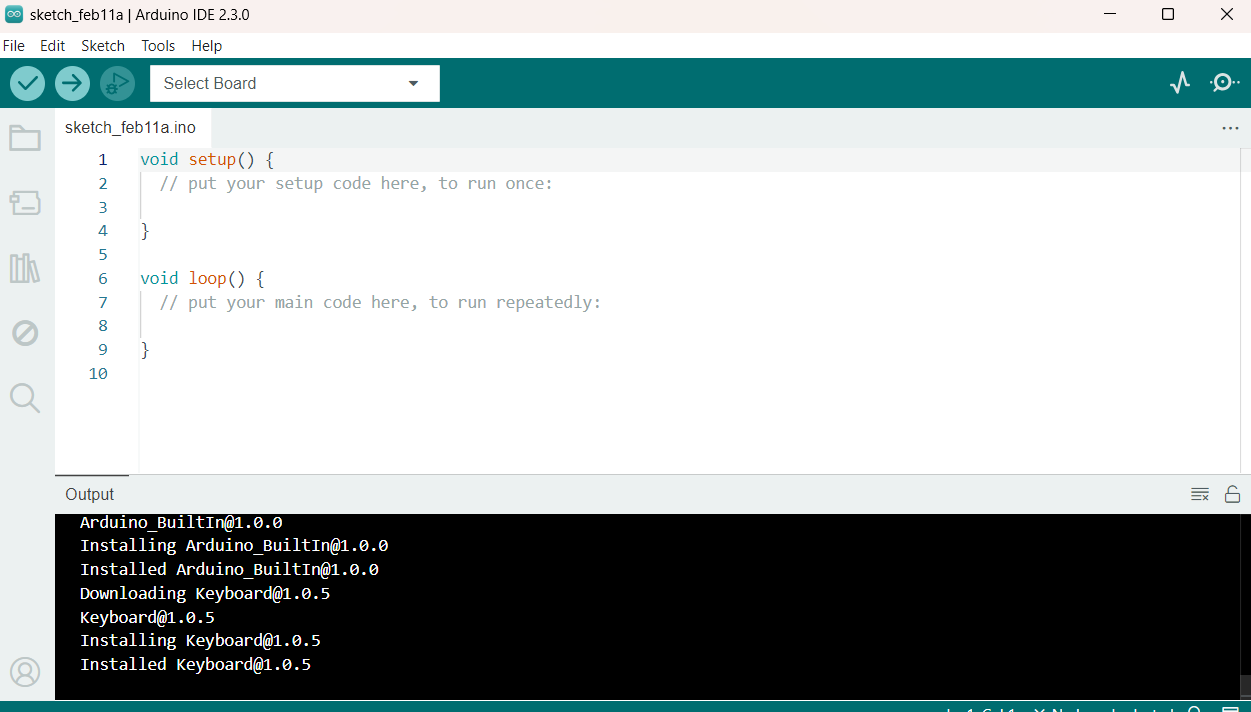
\includegraphics[width=8cm]{Arduino/ArdiunoIDE2/ArduinoIDESketch}
    \caption{\textbf{Arduino IDE Sketch.}}
    \label{fig:Arduino IDE Sketch}		
\end{figure}


It can be seen from the above figure that the basic arduino sketch has two parts. The first part is the function \PYTHON{void setup()} which returns void and we do the intiliaztion such as the output LED color, specifying the core etc. The second part is the function \PYTHON{void loop()} where we define functions which are to be performed through out the loop. These codes are placed between paranthesis \PYTHON{$\{ \}$} and each function has a return type, here it has void return type.


\subsection{Installation (MacOS)}

To install the Arduino IDE, we need to download the latest version from the Arduino webpage \url{https://www.arduino.cc/en/software}. We can select the version based on the operating system we are using. Here we are installing Arduino 2.3.2 for a MacOS(Sonoma 14.4.1) operating system. The set up file name is \FILE{arduino-ide\_2.3.2\_macOS\_64bit.dmg} and the size of it is 1,93,600 KB. The file is in Zip format. If you use Safari it will be automatically extracted. If you use a different browser you may need to extract it manually. The most recent offline arduino IDE 2.3.2 can be seen in Figure ~\ref{fig:ArduinoIDE Create Agent Installation} it is also supportive for all operating systems.

\begin{center}
    
    \includegraphics[width=0.7\linewidth]{Arduino/ArdiunoIDE2/ArduinoIdeCreateAgentInstallation.png}
    %\label{fig:ArduinoIDE Create Agent Installation}
    \captionof{figure}{ArduinoIDE Create Agent Installation}
    \label{fig:ArduinoIDE Create Agent Installation}
\end{center}

\begin{center}
    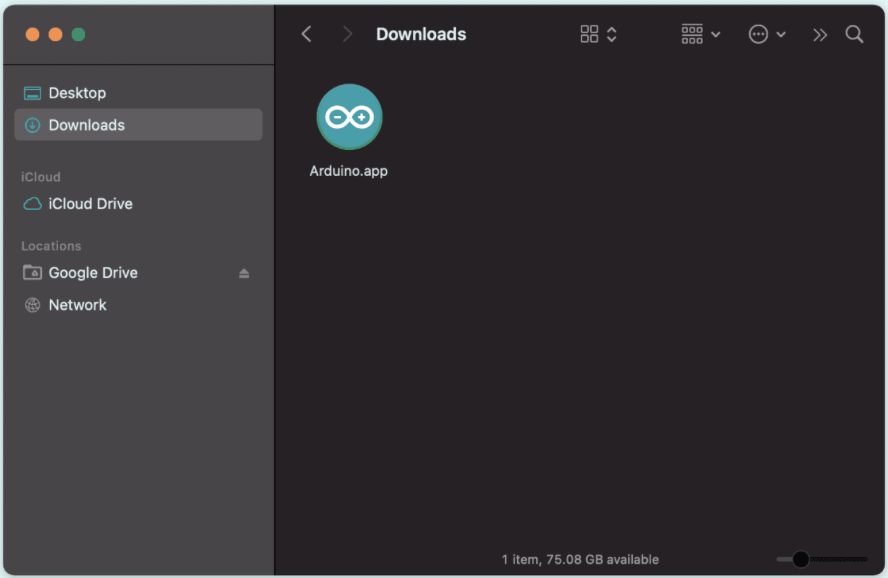
\includegraphics[width=0.7\linewidth]{Arduino/ArdiunoIDE2/OpenTheDownloadFolder.png}
    \captionof{figure}{Open the Downloadf folder}
\end{center}

Copy the Arduino application bundle into the Applications folder (or elsewhere on your computer) then it look like Figure \ref{fig:Copy to the Applications folder}

\begin{center}
    
    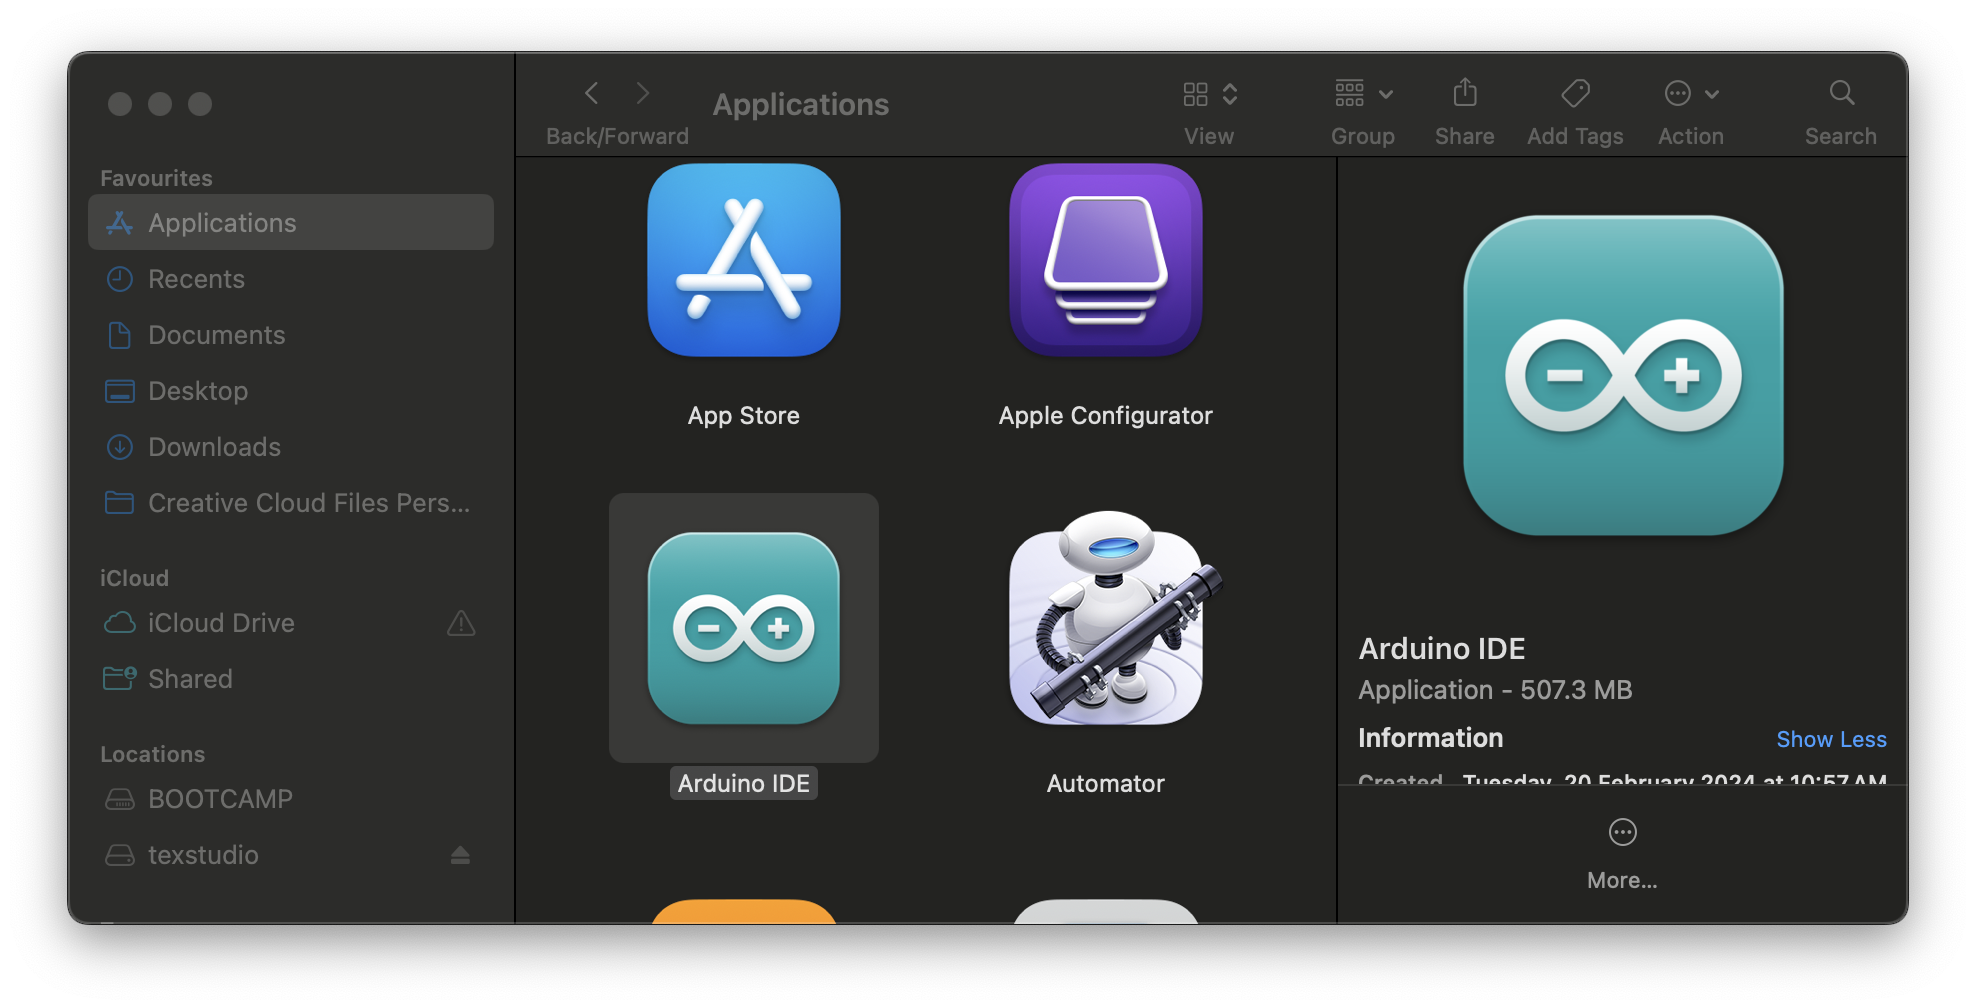
\includegraphics[width=0.7\linewidth]{Arduino/ArdiunoIDE2/CopyToTheApplicationsFolder.png}
    \label{fig:Copy to the Applications folder}
    \captionof{figure}{Copy to the Applications folder}
\end{center}

It can be seen from the Figure \ref{fig:Arduino Sketch} that the basic Arduino sketch has two parts. 

\begin{itemize}
    \item Void setup(): This function returns void and we do the intiliaztion such as the output LED color, specifying the core etc
    \item Void loop(): In this function we define functions which are to be performed throughout the loop. These codes are placed between paranthesis {} and each function has a return type, here it has void return type.
\end{itemize}

\begin{center}
    \label{fig:Arduino Sketch}
    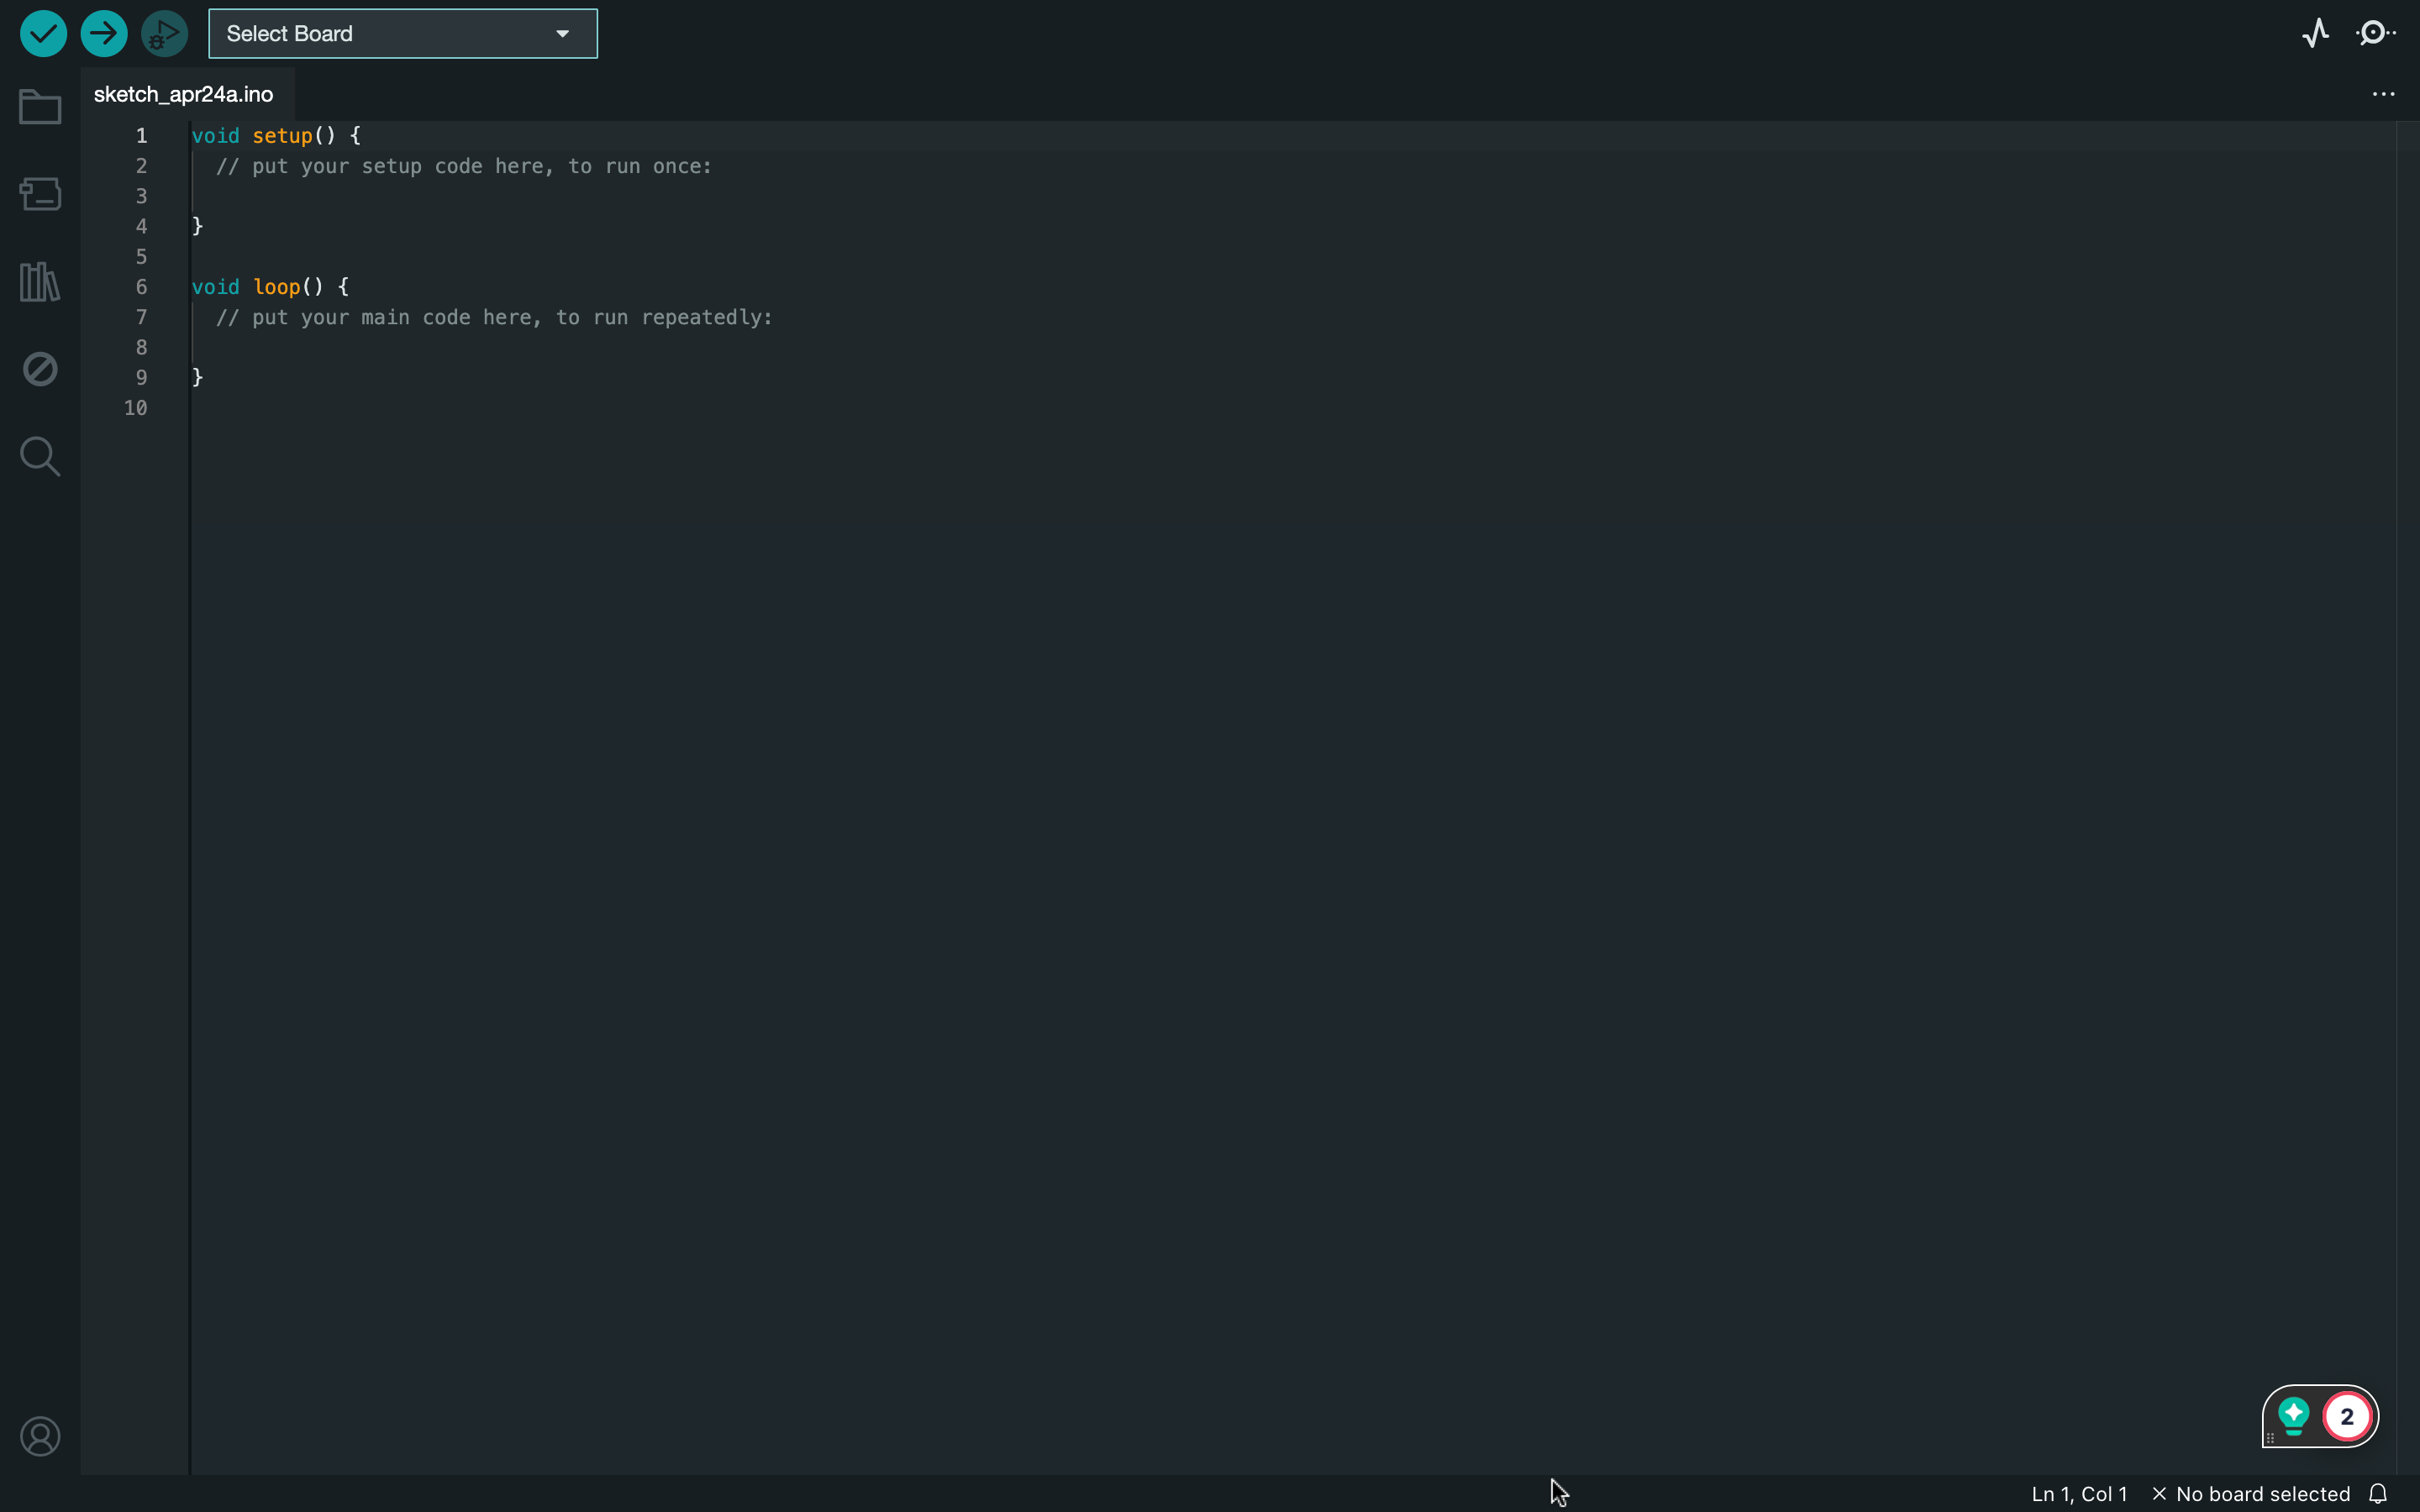
\includegraphics[width=0.7\linewidth]{Arduino/ArdiunoIDE2/ArduinoIDESketch2.png}
    \captionof{figure}{Arduino Sketch}
\end{center}


\subsection{Configuration for the Arduino PortentaH7}

\subsubsection{Introduction}

In this section we will be looking at how to connect the Arduino Portenta H7 with a PC/laptop in order to use the board. Then, we will be going through the first steps of installing the relevant packages to use the Arduino Portenta H7 board and then we will be implementing a basic example sketch from the Arduino IDE.

\subsubsection{Step-wise Configuration}

\begin{enumerate}
    
    \item Connect the Arduino Portenta H7 board to the computer via USB Type-C cable.
    \item Press the reset button twice on the board and the LED on the board starts blinking green as shown in the Figure \ref{fig:Arduino PortentaH7 Connected to a Laptop} indicating that it is ready.
    
    
    
    \item Install the packages in order to use the Arduino Portenta board. To do this search for Portenta in the boards and select \textbf{Arduino Mbed OS Portenta Boards} and click install as shown in Figure \ref{fig:Installation Arduino Mbed OS Portenta Board}. After the installation is done, we can start writing sketches in the IDE.
\end{enumerate}	

\begin{center}
    \label{fig:Installation Arduino Mbed OS Portenta Board}
    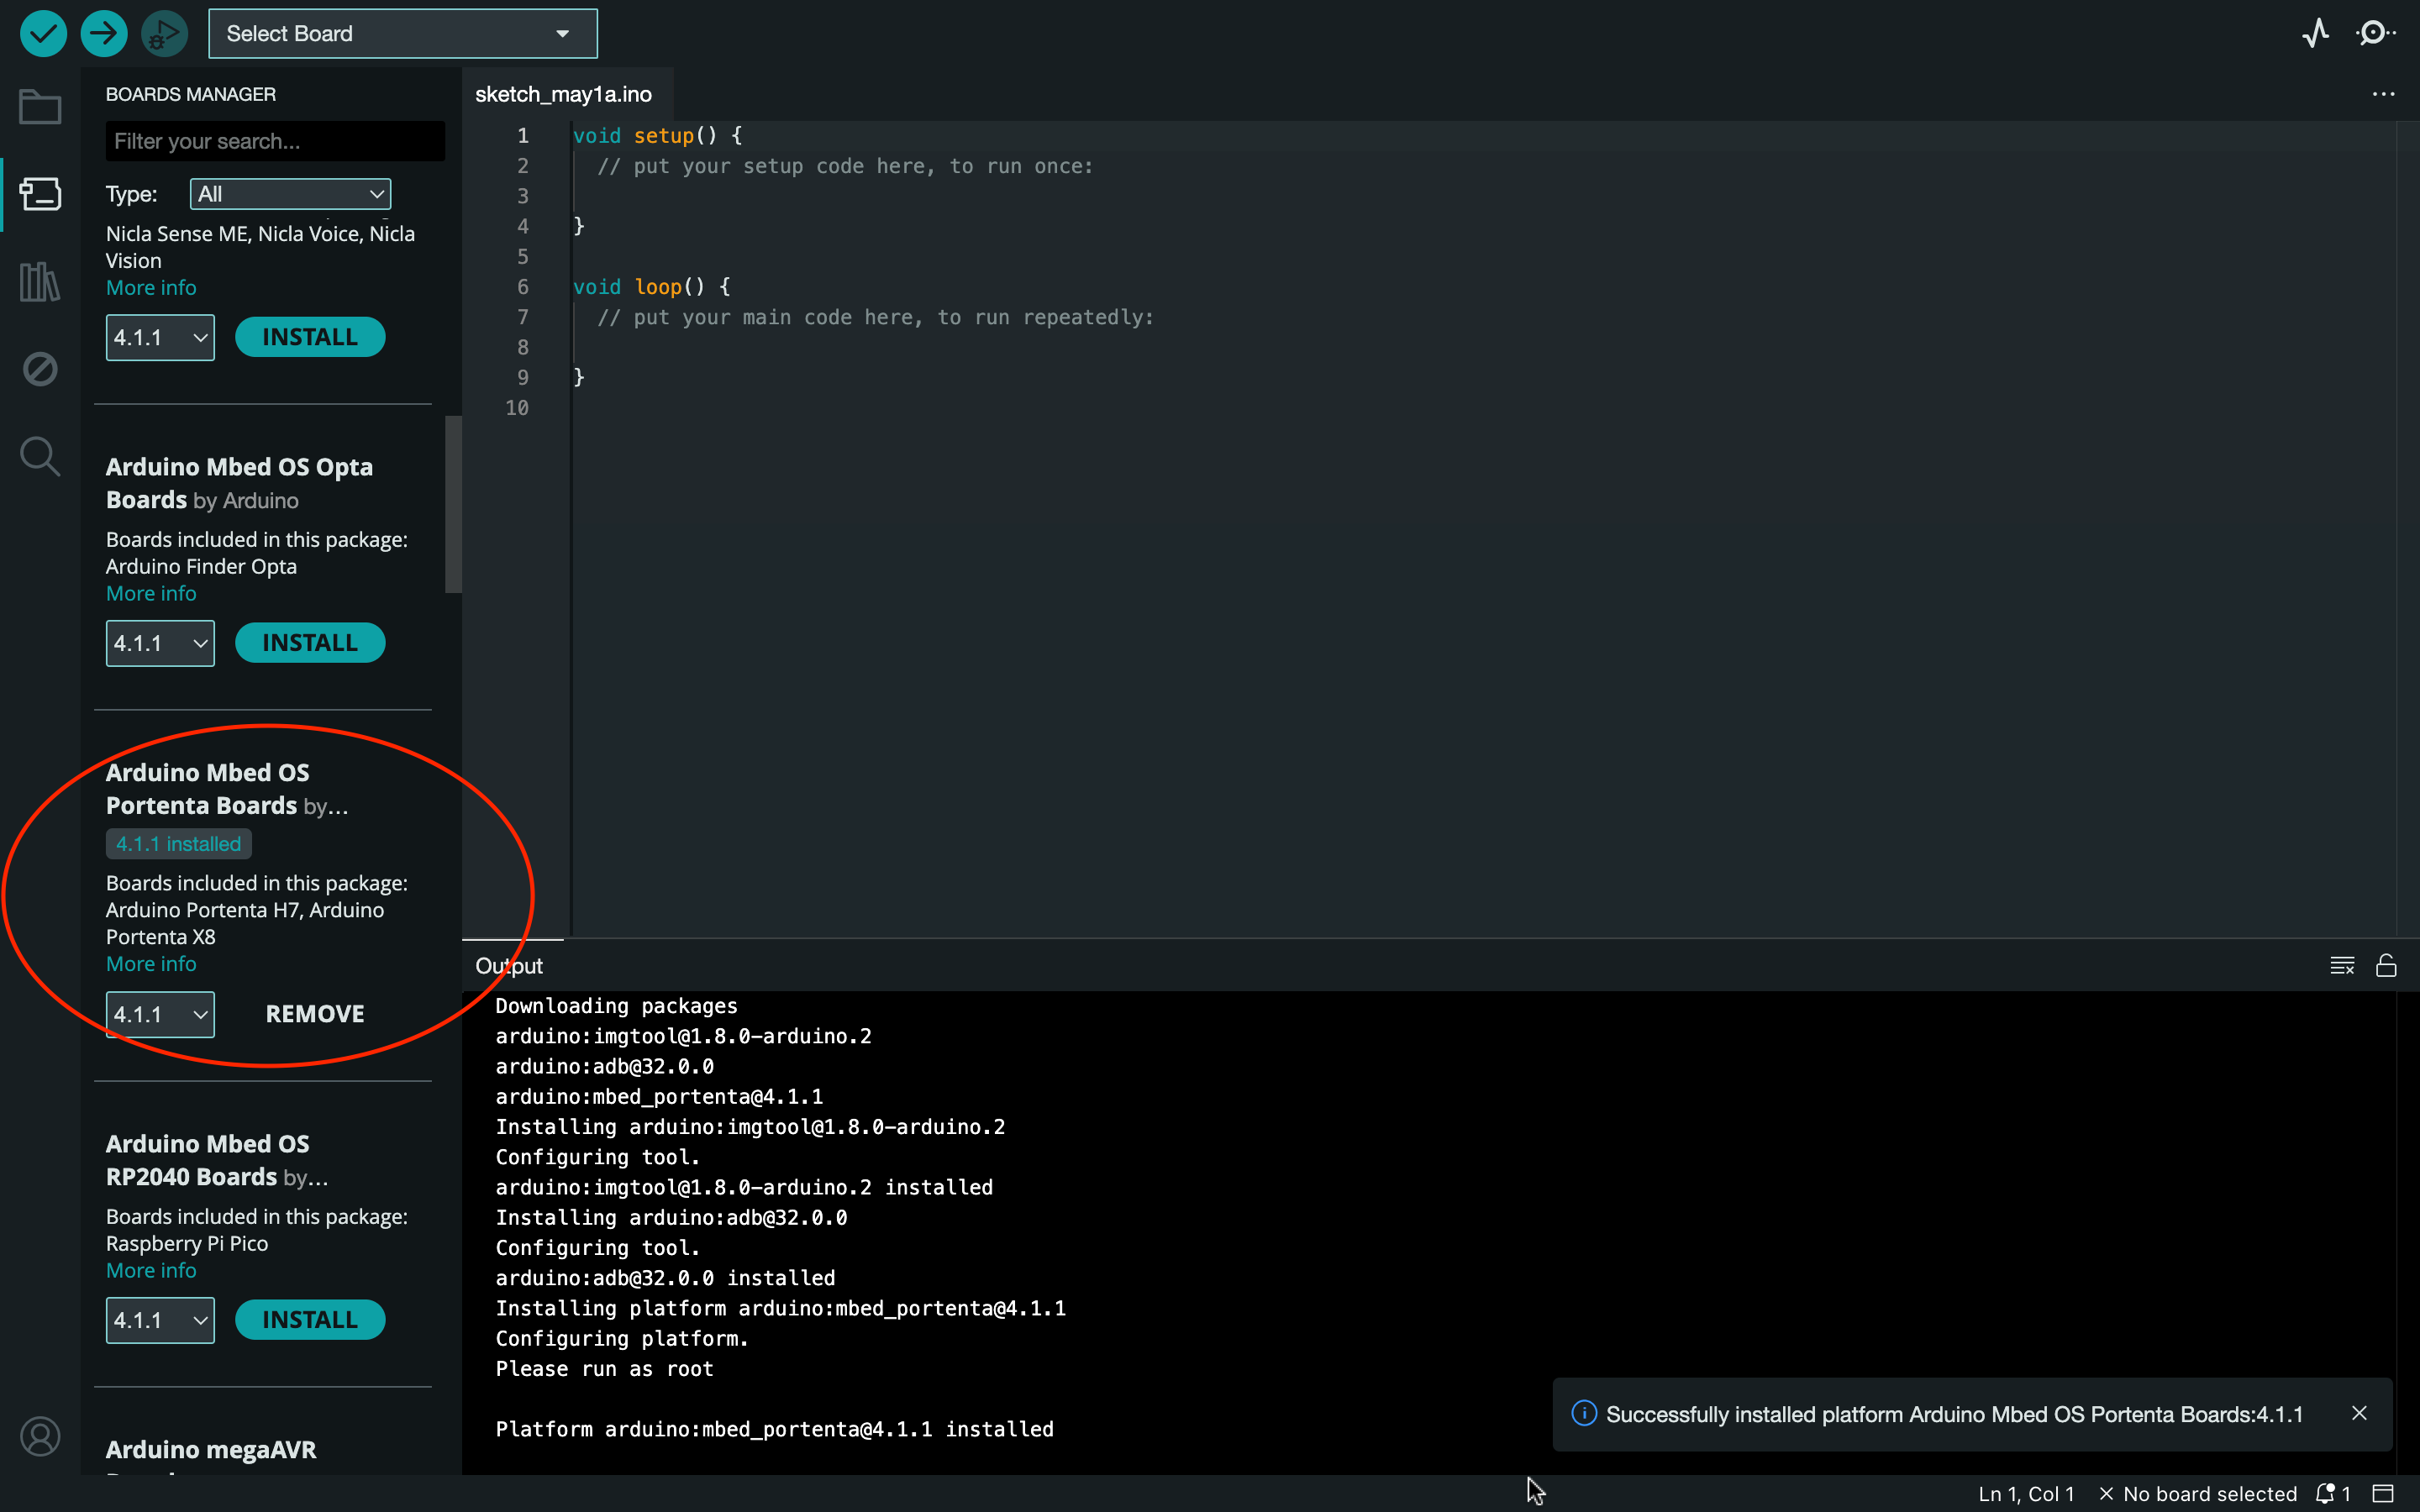
\includegraphics[width=0.7\linewidth]{Arduino/ArdiunoIDE2/ArduinoMbedOSPortentaBoardsInstallation}
    \captionof{figure}{Installation Arduino Mbed OS Portenta Board}
\end{center}


\subsubsection{Example Blink Sketch}

To upload the example sketch, go to File then click on examples and then click on 01.Basics and then select blink as shown in Figure \ref{fig:Example LED-Test}.

\begin{center}
    \label{fig:Arduino PortentaH7 Connected to a Laptop}
    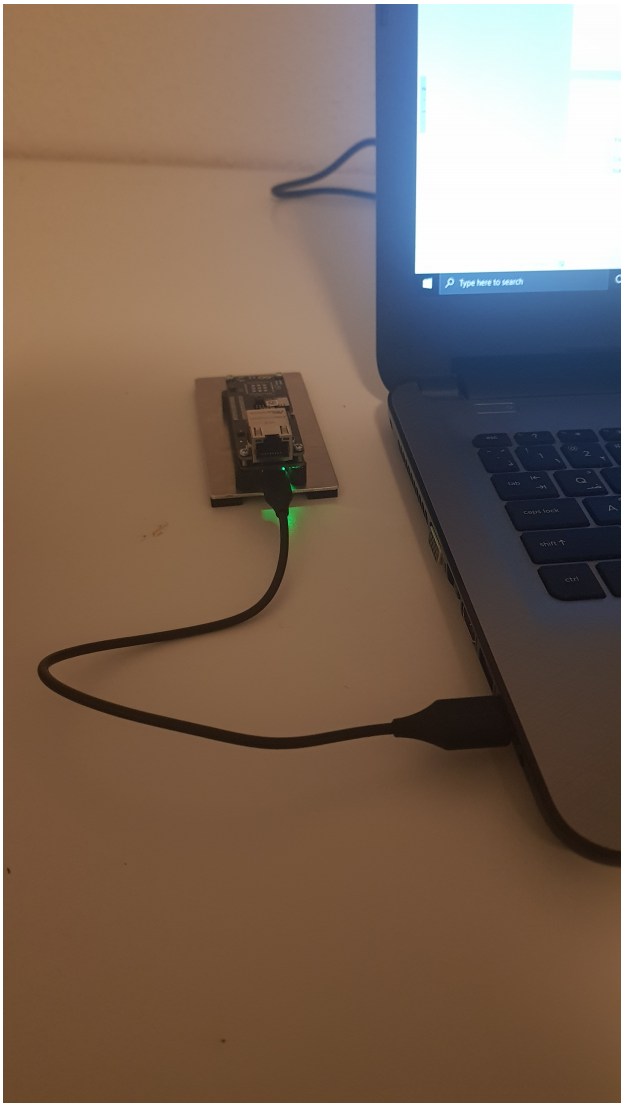
\includegraphics[width=0.7\linewidth]{Arduino/ArdiunoIDE2/ArduinoPortentaH7Connectedtoalaptop}
    \captionof{figure}{Arduino PortentaH7 Connected to a Laptop}
\end{center}

\begin{center}
    \label{fig:Example LED-Test}
    \includegraphics[width=0.7\linewidth]{Arduino/ArdiunoIDE2/MenuBarOptions.png}
    \captionof{figure}{Example LED-Test}
\end{center}


In the program, we initialize LED\_BUILTIN as the output in the setup function. In the loop function we turn on the LED by using digitalWrite() function. Click on upload and wait for it to complete. After the upload is done, the green LED on the board starts blinking with a delay of 1000ms.The blink sketch appears on the screen as shown in Figure \ref{fig:Blink Sketch Compile}.

\begin{center}
    \label{fig:Blink Sketch Compile}
    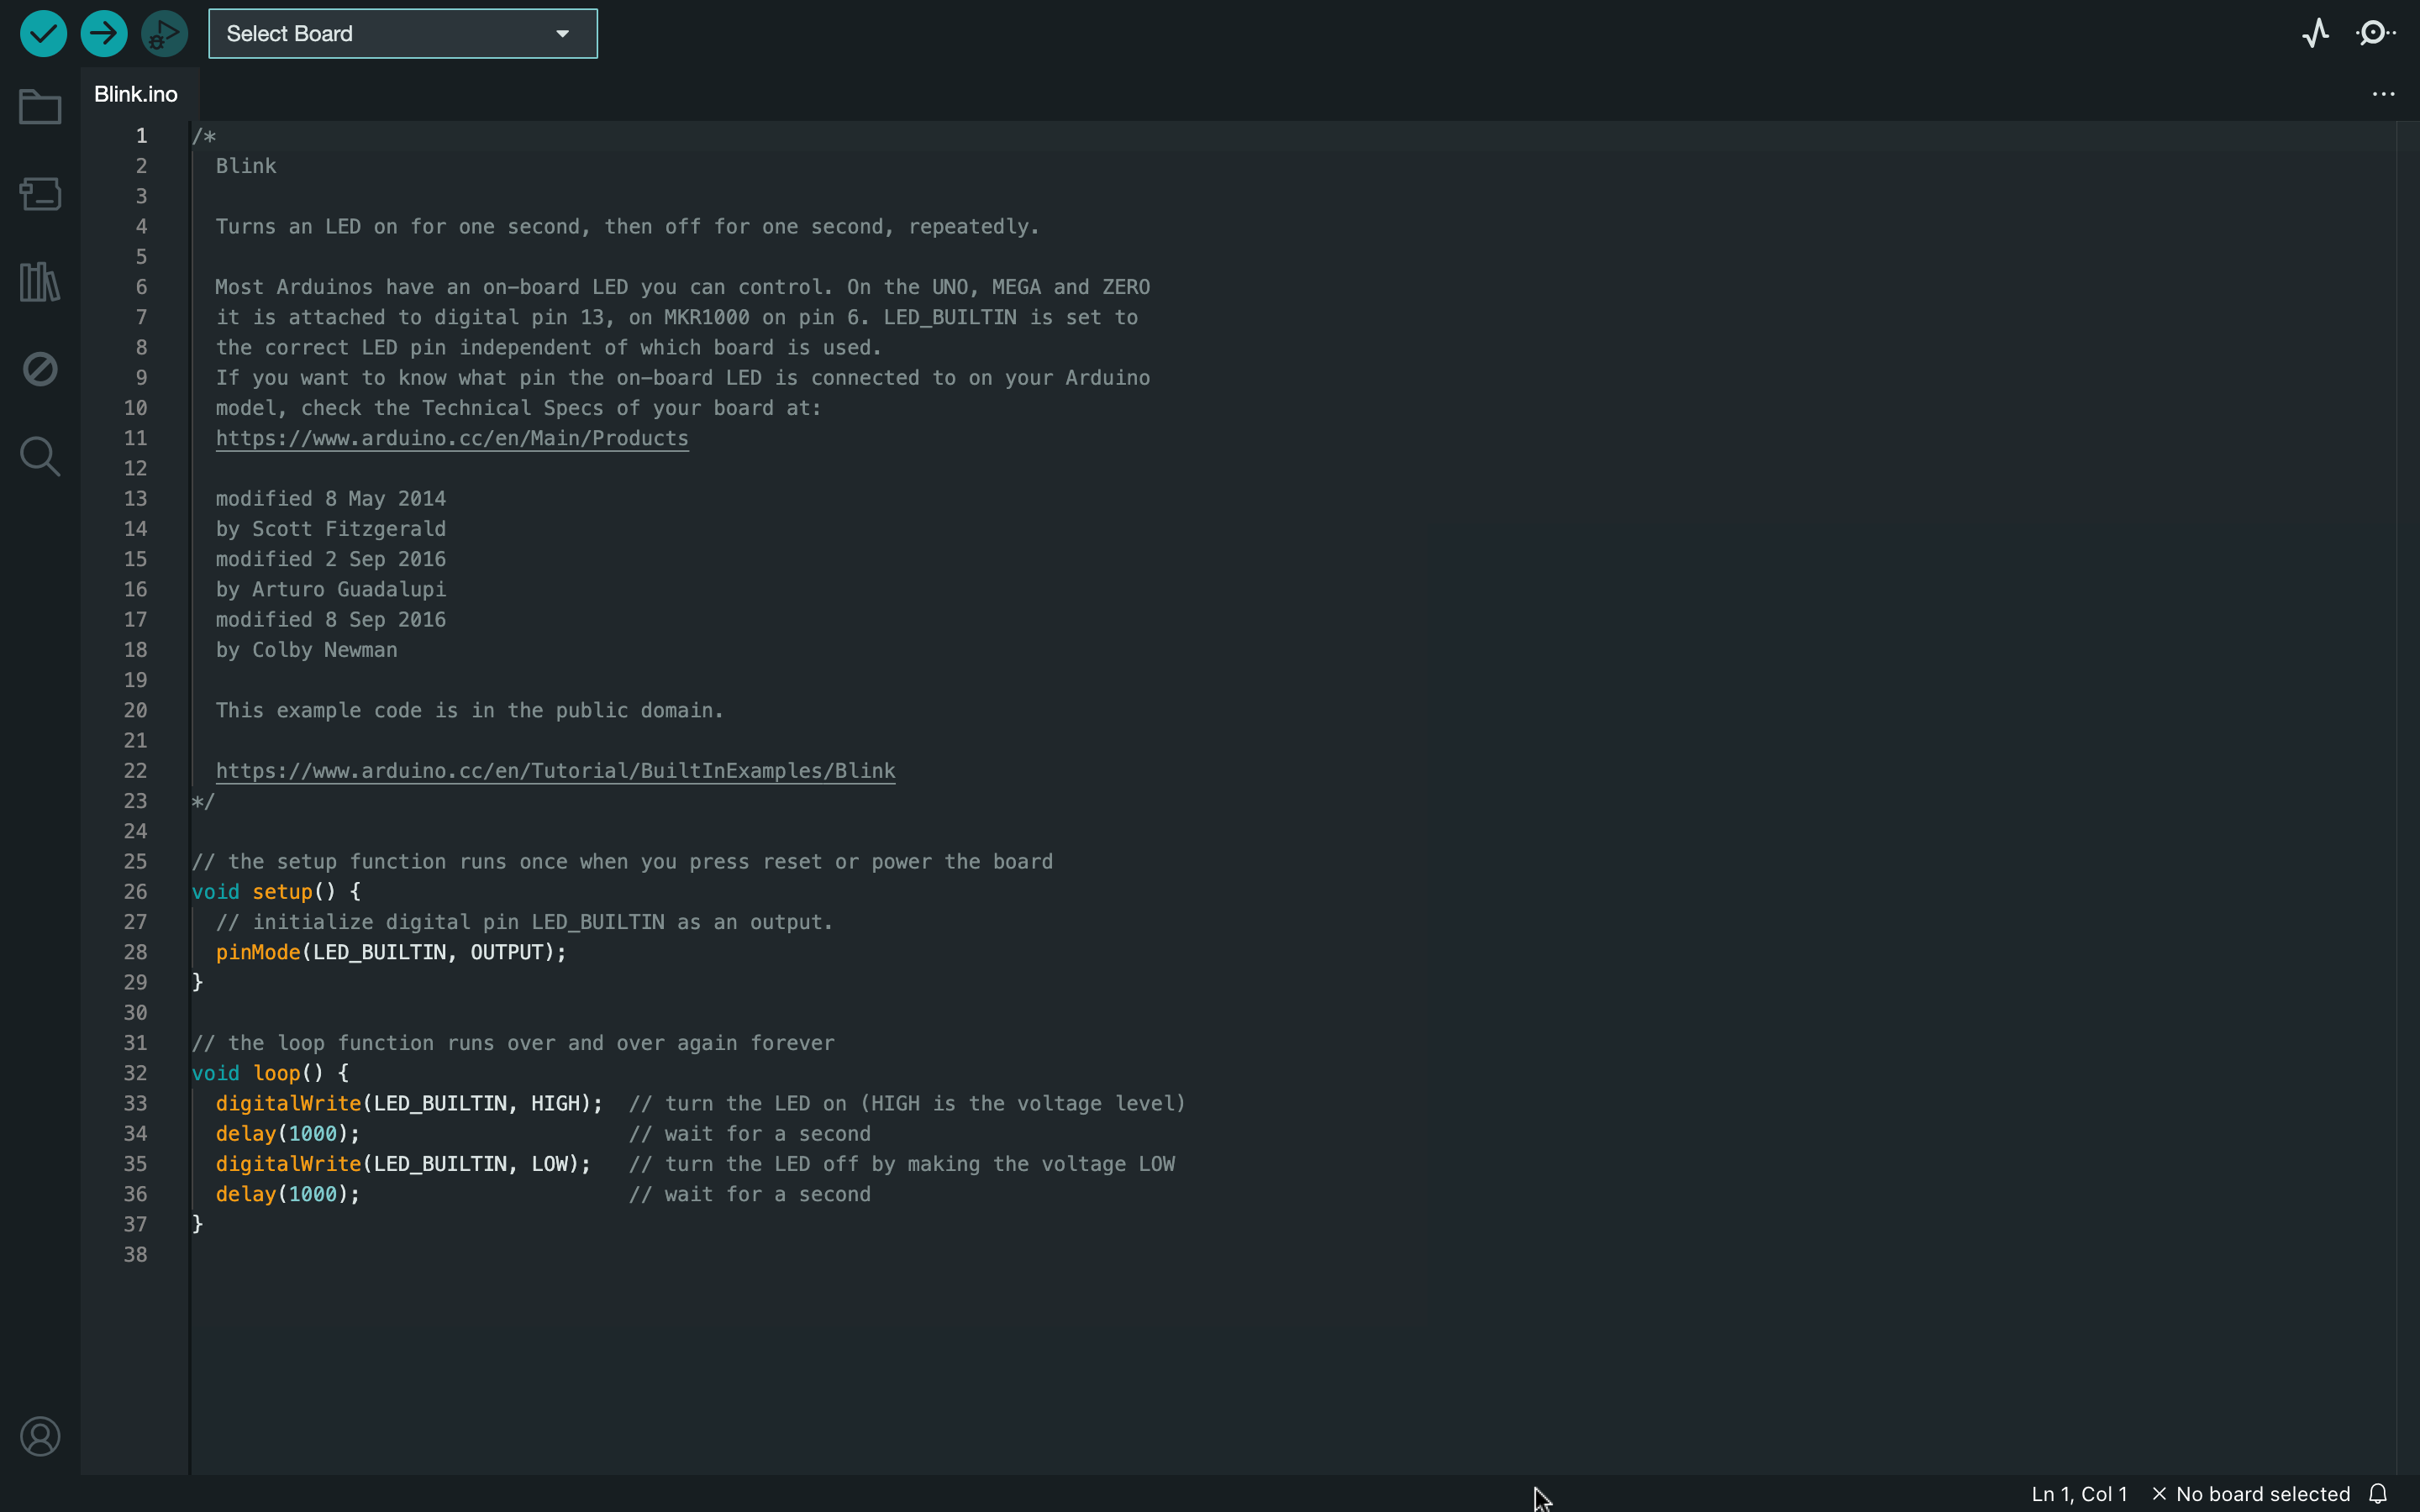
\includegraphics[width=0.7\linewidth]{Arduino/ArdiunoIDE2/CompileBlinkSketch.png}
    \captionof{figure}{Blink Sketch Compile}
\end{center}


\subsection{Configuration for the Arduino Nano 33 BLE Sense}

To program the Arduino Nano 33 BLE Sense in offline state, we need to install one
of the latest arduino IDE on our desktop. After installation, for getting access to
the Arduino nano 33 ble sense board, we need to make configuration in our IDE. By
opening the IDE, go to tool which can be seen on the uper left corner in IDE, in the
tool there is an option for managed board. At this point we need to write our board
name in the search which is Arduino Nano 33 BLE Sense as shown in figure,\ref{fig:Arduino Mbed OS Nano Boards Installation}.Select
the Arduino Mbed OS Boards and install it. The Mbed OS nano board supports also
other nano family boards including Arduino nano 33 ble sense, after installing simply
connect the Arduino Nano 33 BLE Sense to the computer via USB cable.


\begin{figure}[H]\centering
    \includegraphics[width=8cm]{Arduino/ArdiunoIDE2/ArduinoMbedOSNanoBoardsInstallation}
    \caption{\textbf{Arduino Mbed OS Nano Boards Installation.}}
    \label{fig:Arduino Mbed OS Nano Boards Installation}		
\end{figure}



\subsection{Setup}

There are set of examples which are build in Arduino (IDE) for the testing purpose, for checking all the configuration and setting up the board we can open one of the basic LED blink example first as shown in the figure.  \ref{fig:LED-Example Test}.



\begin{figure}[H]\centering
    \includegraphics[width=8cm]{Arduino/ArdiunoIDE2/MenuBarOptions}
    \caption{\textbf{LED-Example Test.}}
    \label{fig:LED-Example Test}		
\end{figure}

This LED-blink example support all the arduino boards, for the checking purposes just need to run this basic example on any arduino embed board and it will blink the LED on our Arduino board after pre-set miliseconds. In the same example folder, there are also number of build in usefull example written in Arduino IDE for embedded boards. These examples are very usefull for getting the basic knowledge about the board and programming.

\subsection{Constraints}

There are some pre-requisite steps need to follow either we need to run the build in example or run by our own written program. By operating the Arduino board with Laptop with the help of USB connection, need to open the Arduino IDE on desktop, it appears a blank arduino environment page just a Void setup and void loop written on it. At this step we need to go to the tool-Arduino board and select the connected board which is Arduino Nano 33 Ble Sense as shown in the figure   \ref{fig:Select the Connected board -here Arduino Nano 33 BLE Sense}

\begin{figure}[H]\centering
    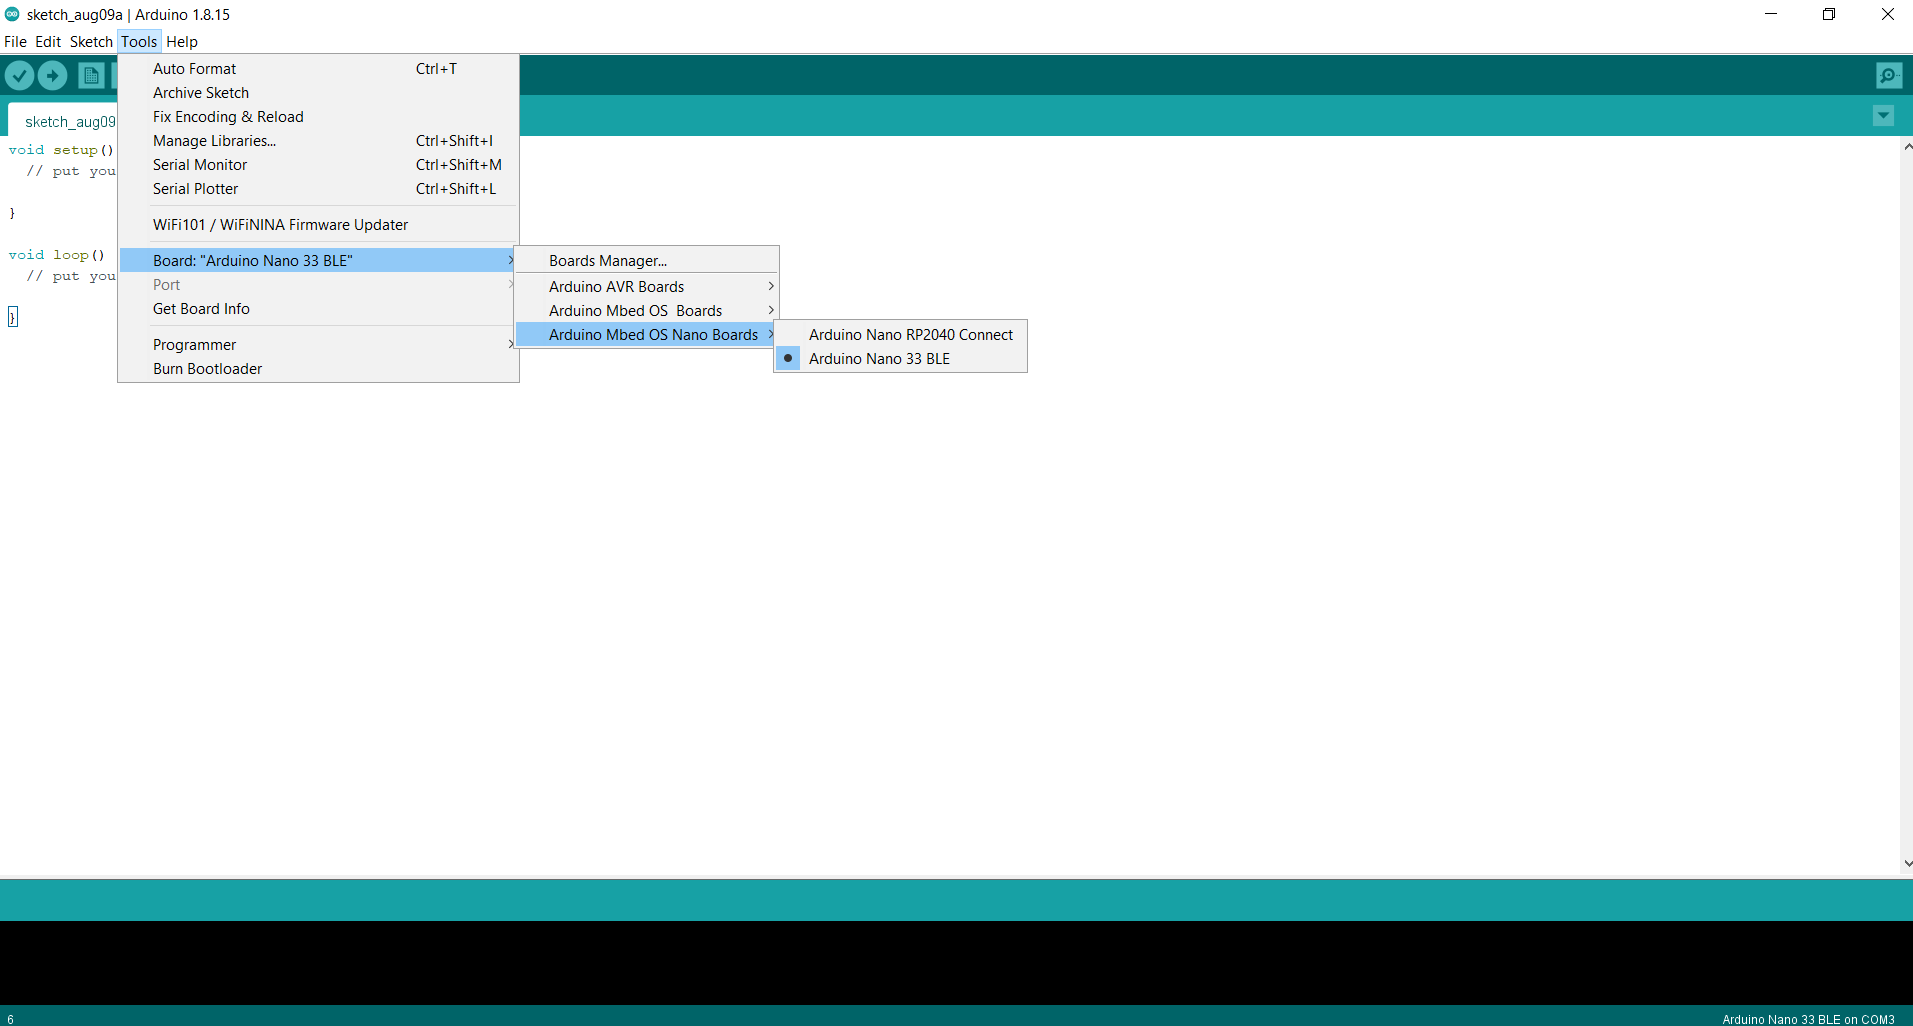
\includegraphics[width=8cm]{Arduino/ArdiunoIDE2/SelectTheConnectedBoardArduinoNano33BLESense}
    \caption{\textbf{Select the Connected board -here Arduino Nano 33 BLE Sense.}}
    \label{fig:Select the Connected board -here Arduino Nano 33 BLE Sense}		
\end{figure}

\subsection{Select the Appropriate Port}

By selecting the Arduino nano 33 BLE sense board, next we need to check the connected port. For doing this, we need to set our arduino borad in Boot setup by clicking the white reset button on arduino as show in figure \ref{fig:Arduino Nano 33 BLE Sense Reset Button}.

\begin{figure}[H]\centering
    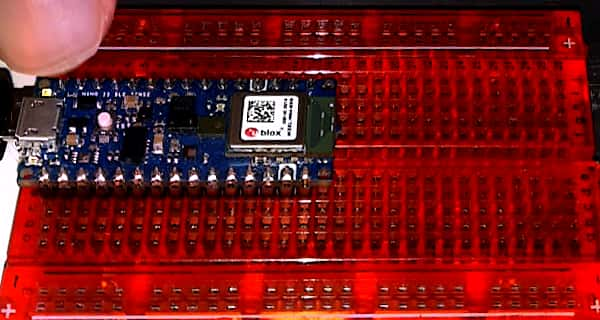
\includegraphics[width=8cm]{Arduino/ArdiunoIDE2/ArduinoNano33BLESenseResetButton}
    \caption{\textbf{Arduino Nano 33 BLE Sense Reset Button.}}
    \label{fig:Arduino Nano 33 BLE Sense Reset Button}		
\end{figure}

By clicking the white reset button, the arduino borad will be in boot setup and make sure to check the orange LED glows as shown in the figure \ref{fig:Arduino Nano 33 BLE Sense Orange LED Glow}

\begin{figure}[H]\centering
    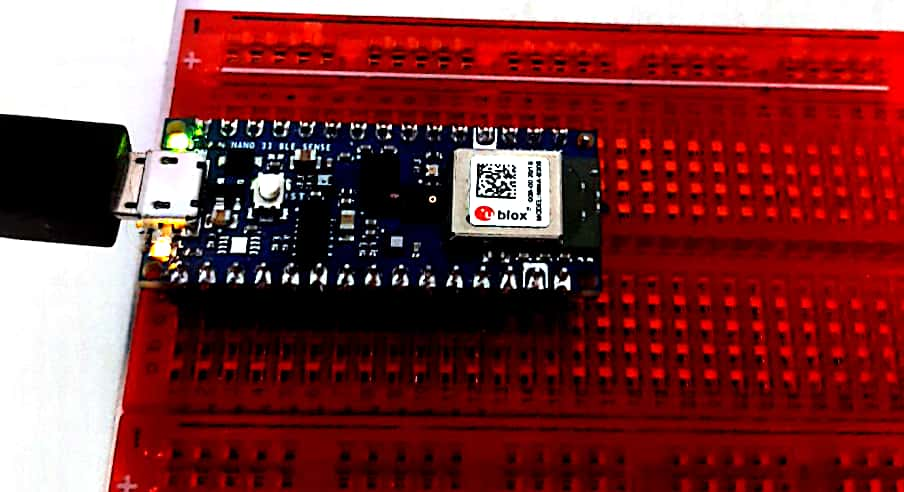
\includegraphics[width=8cm]{Arduino/ArdiunoIDE2/ArduinoNano33BLESenseOrangeLEDGlow}
    \caption{\textbf{Arduino Nano 33 BLE Sense Orange LED Glow.}}
    \label{fig:Arduino Nano 33 BLE Sense Orange LED Glow}		
\end{figure}

After successfully applying the above mention step, next we need to select the connectedport before upload the program. For this, go to tool select arduino port and make sure to check it available port for uploading the program as shown in figure \ref{fig:Select Available Port for Uploading Arduino Sketch}

\begin{figure}[H]\centering
    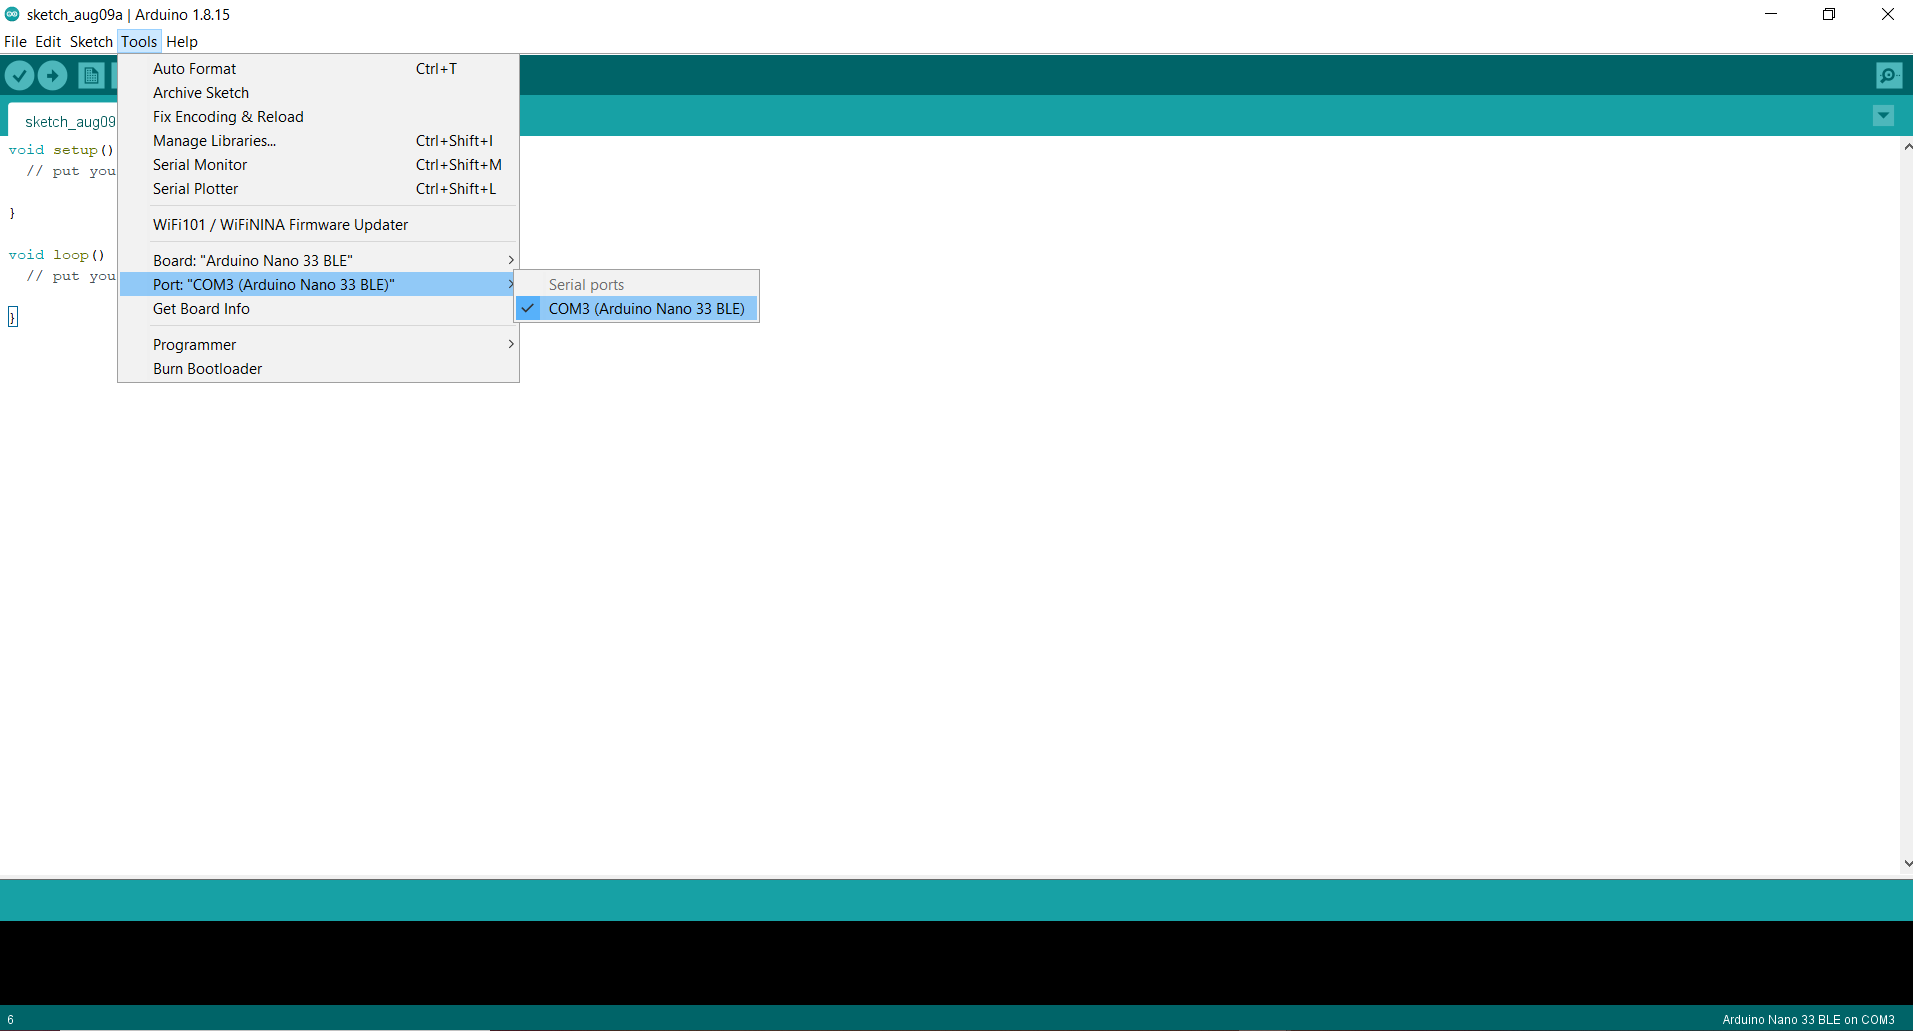
\includegraphics[width=8cm]{Arduino/ArdiunoIDE2/SelectAvailablePortForUploadingArduinoSketch}
    \caption{\textbf{Select Available Port for Uploading Arduino Sketch.}}
    \label{fig:Select Available Port for Uploading Arduino Sketch}		
\end{figure}

\subsection{Upload Code in Arduino Board}\label{uploadcode}

By making sure to select the appropriate port, it’s time to upload the Arduino program. There are five icons (verify, upload, new, open, save) below the file section, before uploading the program the best practice is to verify the program first, it show us if there are any error or warning in the program exist or not. By successfully verifying
the program we can safely upload the program by click the upload button in the top below the file section as shown in figure. \ref{fig:Upload the Program in Arduino board}

\begin{figure}[H]\centering
    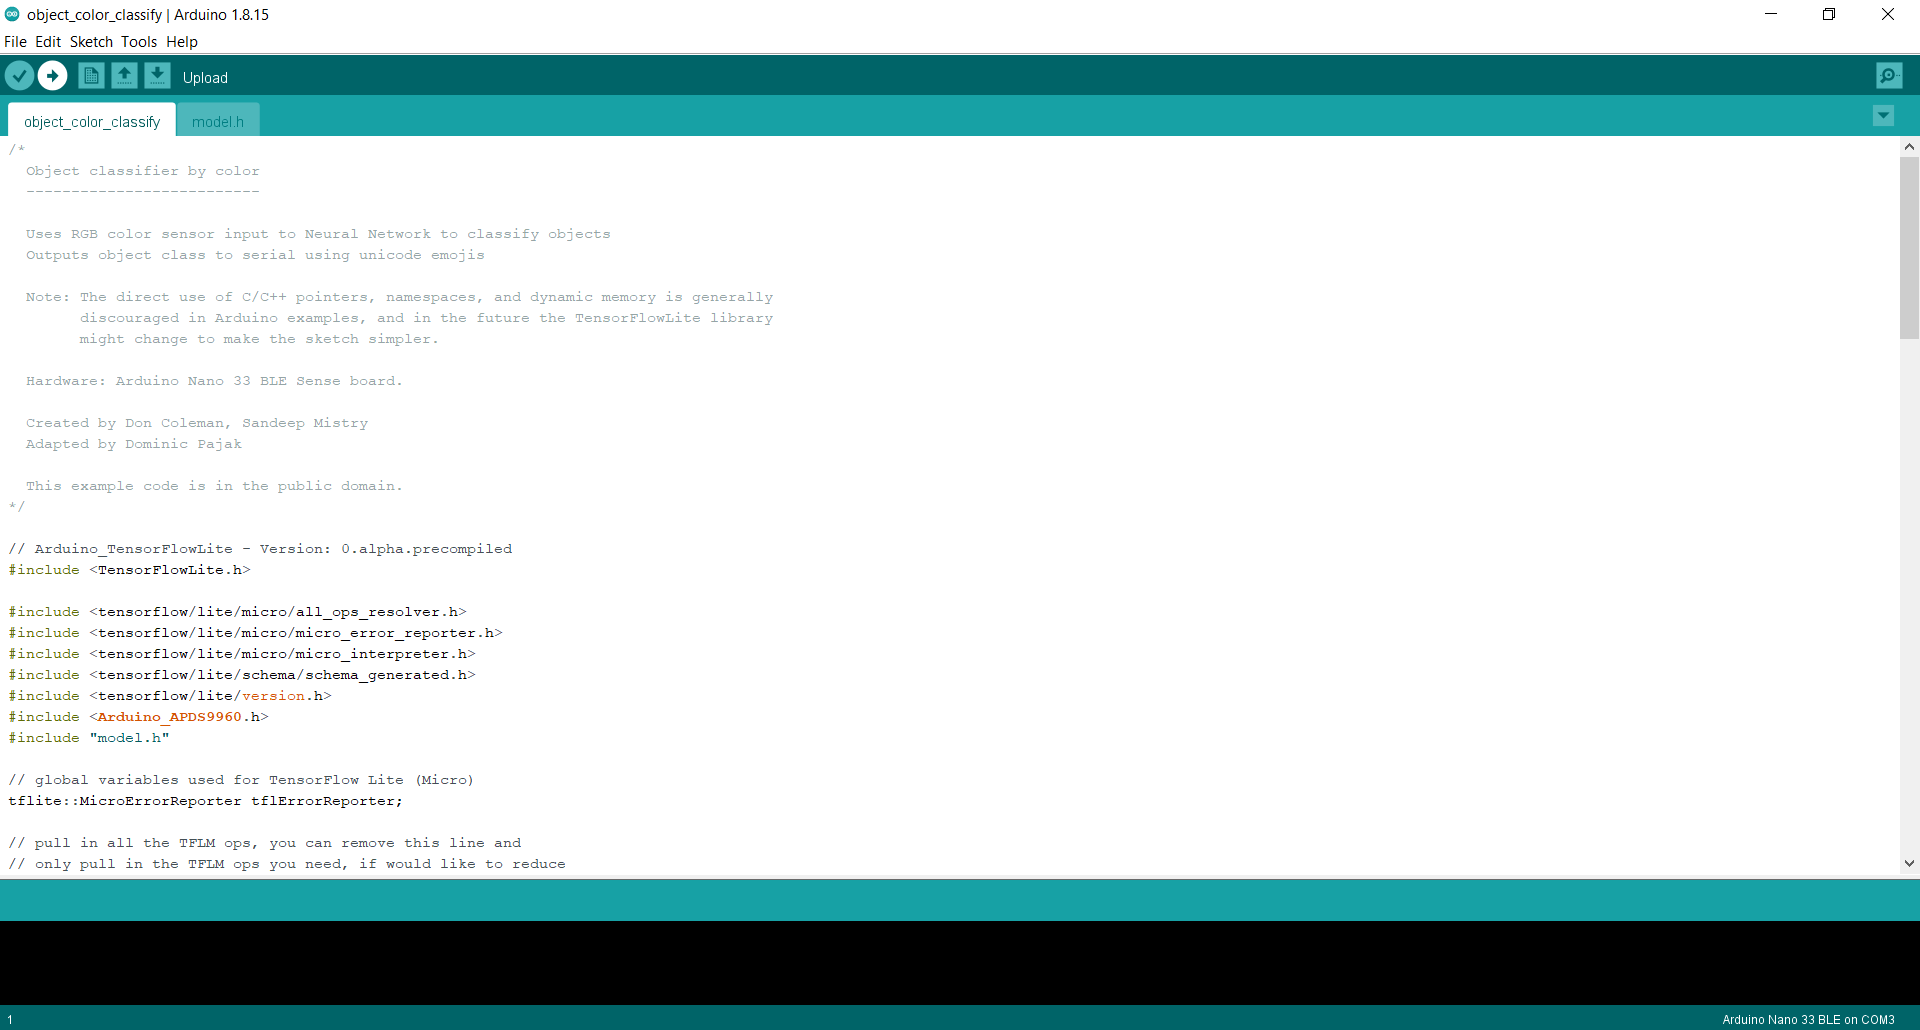
\includegraphics[width=8cm]{Arduino/ArdiunoIDE2/UploadTheProgramInArduinoBoard}
    \caption{\textbf{Upload the Program in Arduino board.}}
    \label{fig:Upload the Program in Arduino board}		
\end{figure}

After uploading, the code will compile and if there is any issue in our program it will pop up in the bottom black window as well.
After successfully uploading and compiling the code in Arduino board, it also require to change the port again as we did it previously. Go to tool select arduino port and
make sure to check the port again as shown in figure \ref{fig:Setting the Port} by getting output in the
serial monitor.

\begin{figure}[H]\centering
    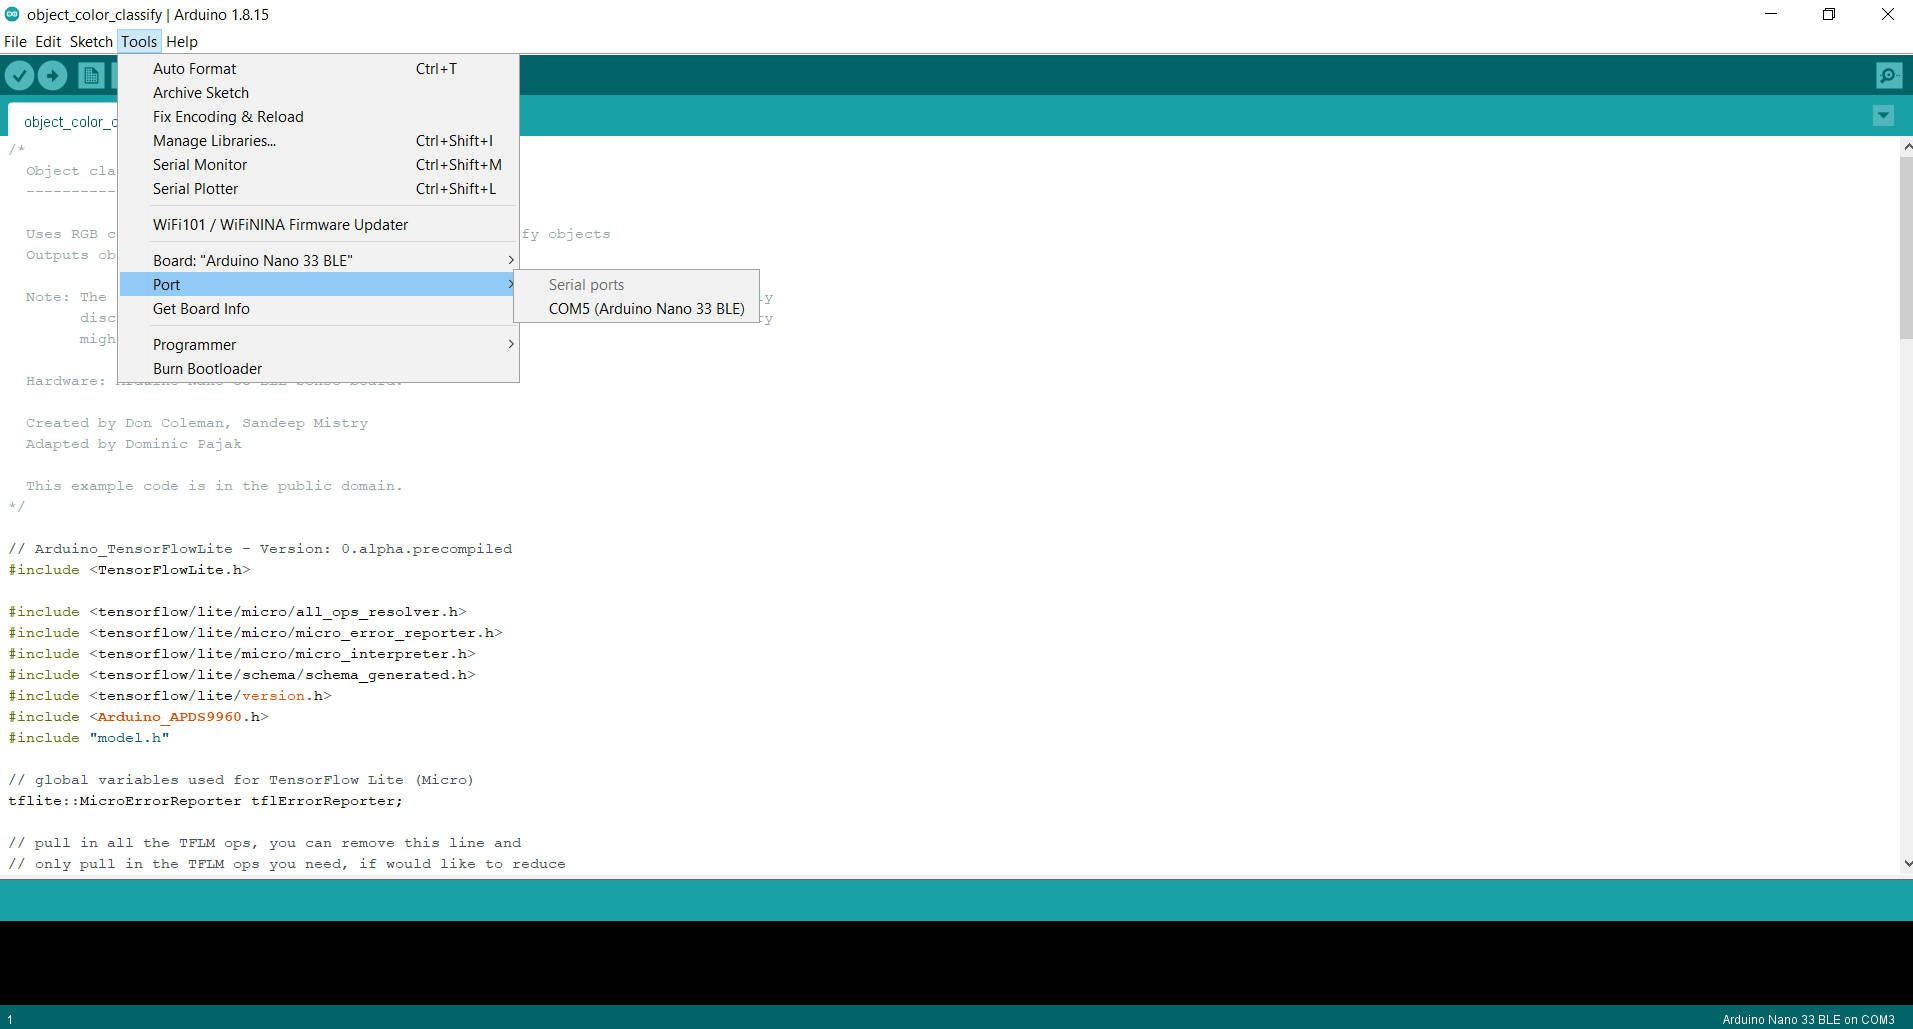
\includegraphics[width=8cm]{Arduino/ArdiunoIDE2/SettingThePort}
    \caption{\textbf{Setting the Port.}}
    \label{fig:Setting the Port}		
\end{figure} 


\subsection{Data Quality}

The Arduino Integrated Development Environment (IDE) is a key component in the Magic Wand project with Arduino Nano 33 BLE Sense. Here's a detailed explanation of its quality aspects. \cite{Fezari:2018}

\begin{enumerate}
    \item \textbf{Ease of Use}: The Arduino IDE is user-friendly and designed to be easy to use for beginners, while also providing advanced features for experienced users.
    
    \item \textbf{Cross-Platform Compatibility}: The Arduino IDE is compatible with Windows, macOS, and Linux, making it accessible to a wide range of users.
    
    \item \textbf{Open-Source}: The Arduino IDE is open-source, which means its source code is freely available. This allows for community contributions, leading to continuous improvements and updates.
    
    \item \textbf{Support for Multiple Boards}: The Arduino IDE supports not only the Arduino Nano 33 BLE Sense but also a wide range of other Arduino boards.
    
    \item \textbf{Built-In Code Editor}: The Arduino IDE comes with a built-in code editor that provides features like syntax highlighting and automatic indentation, making it easier to write and debug code.
    
    \item \textbf{Library Manager}: The Arduino IDE includes a Library Manager that makes it easy to install and manage libraries. This is particularly useful for the Magic Wand project, which requires libraries like TensorFlow Lite for Microcontrollers.
    
    \item \textbf{Serial Monitor}: The Arduino IDE includes a Serial Monitor that allows you to monitor data sent from the Arduino Nano 33 BLE Sense in real-time. This is crucial for the Magic Wand project, as it allows you to monitor the gesture recognition process.
    
    \item \textbf{Community Support}: The Arduino IDE has a large and active community. This means you can find a wealth of tutorials, guides, and troubleshooting advice online.
\end{enumerate}


\subsection{Data Quantity}
Magic Wand project with Arduino Nano 33 BLE Sense, “Data Quantity” in the software description of the Arduino IDE refers to the amount of data that the software can handle or process. Here’s a detailed explanation:
\begin{enumerate}
    \item \textbf{Code Size}: The Arduino IDE needs to handle the code for the Magic Wand project. This includes the code for collecting and processing sensor data, running the machine learning model, and any additional functionality.
    
    \item \textbf{Library Size}: The Arduino IDE also needs to handle various libraries that are used in the project. This includes the TensorFlow Lite for Microcontrollers library, which is used to run the machine learning model on the Arduino Nano 33 BLE Sense.
    
    \item \textbf{Sensor Data}: The Arduino IDE needs to handle the sensor data that is collected by the Arduino Nano 33 BLE Sense. In one experiment, a window size of 2 seconds was used, which means 200 rows of accelerometer data or 600 values of x, y, and z acceleration axis were fed into the model.\cite{Fezari:2018}
    
    \item \textbf{Model Data}: The Arduino IDE needs to handle the data of the machine learning model. This includes the model parameters and the model output.
    
    \item \textbf{Data Transmission}: The Arduino IDE also handles data transmission between the Arduino Nano 33 BLE Sense and the computer. This includes uploading the program to the board and transmitting sensor data and model output to the computer for monitoring.
\end{enumerate}

\subsection{Data Types}

\begin{itemize}
    \item \textbf{Magic Wand Project with Arduino Nano 33 BLE Sense:} This project involves using TensorFlow Lite for Microcontrollers to run a deep learning model on the Arduino Nano 33 BLE. The microcontroller is turned into a digital "magic wand" that can recognize various gestures.\cite{Fezari:2018}
    
    \item \textbf{Software Components:}
    \begin{itemize}
        \item \textbf{TensorFlow Lite For Microcontrollers:} This is an optimized version of TensorFlow, targeted to run TensorFlow models on tiny, low-powered hardware such as microcontrollers. It doesn't require operating system support, any standard C or C++ libraries, or dynamic memory allocation.
        \item \textbf{Arduino IDE:} This is the software used to write and upload computer code to the physical board.
    \end{itemize}
    
    \item \textbf{Data Types:} You'll likely be working with arrays to store the sensor data, and you'll use TensorFlow Lite's data types for the model's input and output. The exact data types will depend on your specific implementation and the requirements of the TensorFlow Lite model.
\end{itemize}


\begin{enumerate}
    \item \textbf{Numeric Data Types:}
    \begin{itemize}
        \item Identify the numeric data types used, such as integers, floating-point numbers, or doubles.
        \item Describe the range and precision of each numeric data type.
    \end{itemize}
    
    \item \textbf{Text Data Types:}
    \begin{itemize}
        \item Specify if the software handles text data, such as strings or characters.
        \item Discuss any character encoding or formatting requirements.
    \end{itemize}
    
    \item \textbf{Sensor Data Types:}
    \begin{itemize}
        \item If interacting with sensors, specify the types of sensor data used.
        \item Describe the format and units of measurement for each sensor data type.
    \end{itemize}
    
    \item \textbf{Custom Data Types:}
    \begin{itemize}
        \item Discuss any custom data types defined in the software, such as structs or classes.
        \item Explain the purpose and structure of each custom data type.
    \end{itemize}
    
    \item \textbf{Data Conversion and Casting:}
    \begin{itemize}
        \item If data conversion or casting operations are performed, describe how different data types are converted or casted.
    \end{itemize}
    
    \item \textbf{Data Representation:}
    \begin{itemize}
        \item Explain how data is represented, including binary, hexadecimal, or other representations.
    \end{itemize}
\end{enumerate}



\subsection{Data Structure}

\begin{itemize}
    \item \textbf{Magic Wand Project with Arduino Nano 33 BLE Sense:}  project involves using TensorFlow Lite for Microcontrollers to run a deep learning model on the Arduino Nano 33 BLE. The microcontroller is turned into a digital "magic wand" that can recognize various gestures.\cite{Harris:2023}
    
    \item \textbf{Data Structures:}
    \begin{itemize}
        \item \textbf{Sensor Data:} The Arduino Nano 33 BLE Sense collects sensor data, which is multidimensional and complex. This data is typically stored in arrays or similar data structures for processing.
        \item \textbf{Model Input and Output:} The sensor data is passed to the TensorFlow Lite model as input, and the model outputs a simple classification. The exact data structures for these will depend on the requirements of your TensorFlow Lite model.
        \item \textbf{Gesture Recognition:} The project involves recognizing gestures, which are classified into different categories. You might use data structures like enumerations or similar to represent these different categories.
    \end{itemize}
\end{itemize}




\begin{enumerate}
    \item \textbf{Arrays:} Used to store a collection of data items of the same type. Example: storing sensor readings over time, storing LED brightness levels.
    
    \item \textbf{Structures (\texttt{struct}):} Allows grouping multiple variables of different types under a single name. Example: defining a struct to hold sensor data (e.g., temperature, humidity).
    
    \item \textbf{Classes:} Used for creating user-defined data types with properties and methods. Example: defining a class for managing gestures detected by the wand.
    
    \item \textbf{Linked Lists:} Data structures consisting of a sequence of elements where each element points to the next element. Example: implementing a linked list to manage a queue of actions to perform.
    
    \item \textbf{Stacks:} Last in, first out (LIFO) data structures where elements are inserted and removed from the same end. Example: using a stack to manage function calls or nested operations.
    
    \item \textbf{Queues:} First in, first out (FIFO) data structures where elements are inserted at the end and removed from the front. Example: implementing a queue for handling incoming commands or tasks.
    
    \item \textbf{Trees:} Hierarchical data structures consisting of nodes connected by edges. Example: representing hierarchical data such as menu structures or organizational charts.
\end{enumerate}



\subsection{Conclusions}
\subsubsection{Output Window (Serial Monitor)}
Serial Monitor is the another window on the Arduino IDE, which shows the Input/Output of our program and results appear on it as per the required output. For getting
access to Serial monitor, we need to go extreme right in the Arduino IDE, the small
circle pop up when we reach it is the serial monitor as show in the figure.\ref{fig:Serial Monitor Icon}
\begin{figure}[H]\centering
    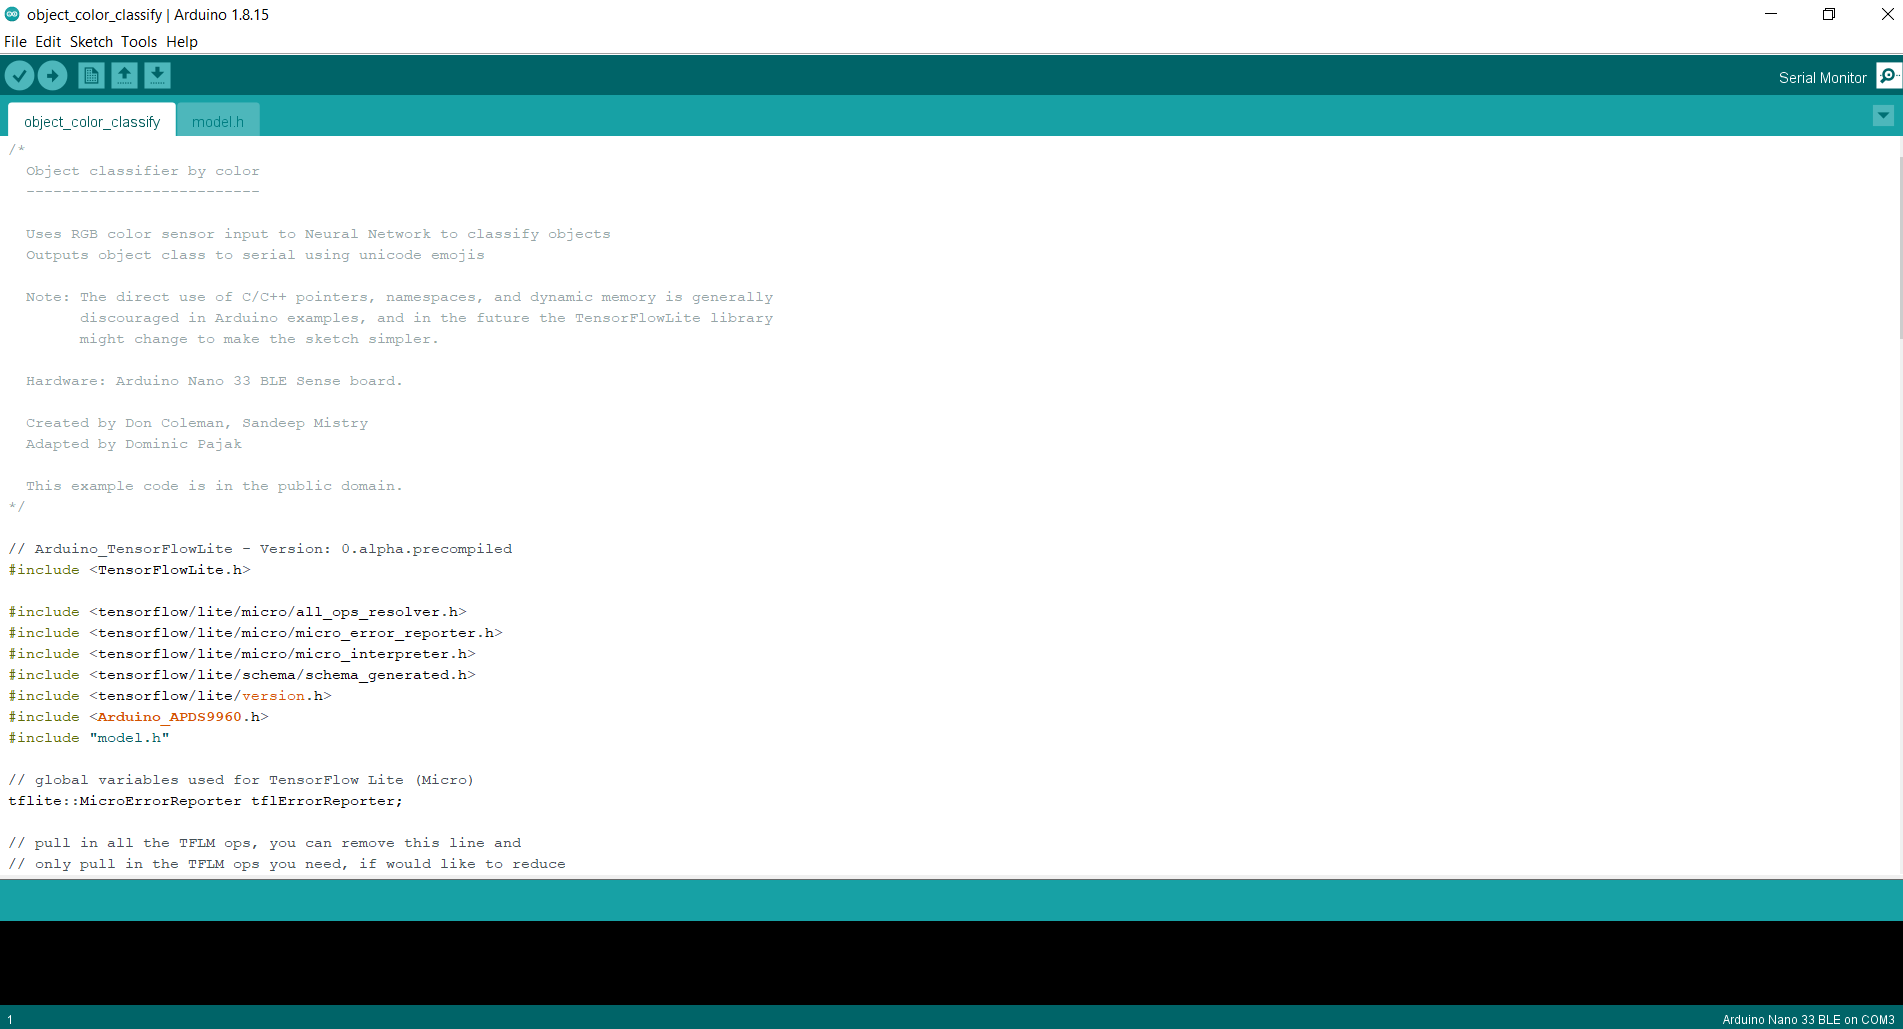
\includegraphics[width=8cm]{Arduino/ArdiunoIDE2/SerialMonitorIcon}
    \caption{\textbf{Serial Monitor Icon.}}
    \label{fig:Serial Monitor Icon}		
\end{figure} 
The Final results, all the variables, input, sensor values are shown in the serial monitor
the (Output Window) as shown in the figure\ref{fig:Output Window} by clicking the serial monitor button.
\begin{figure}[H]\centering
    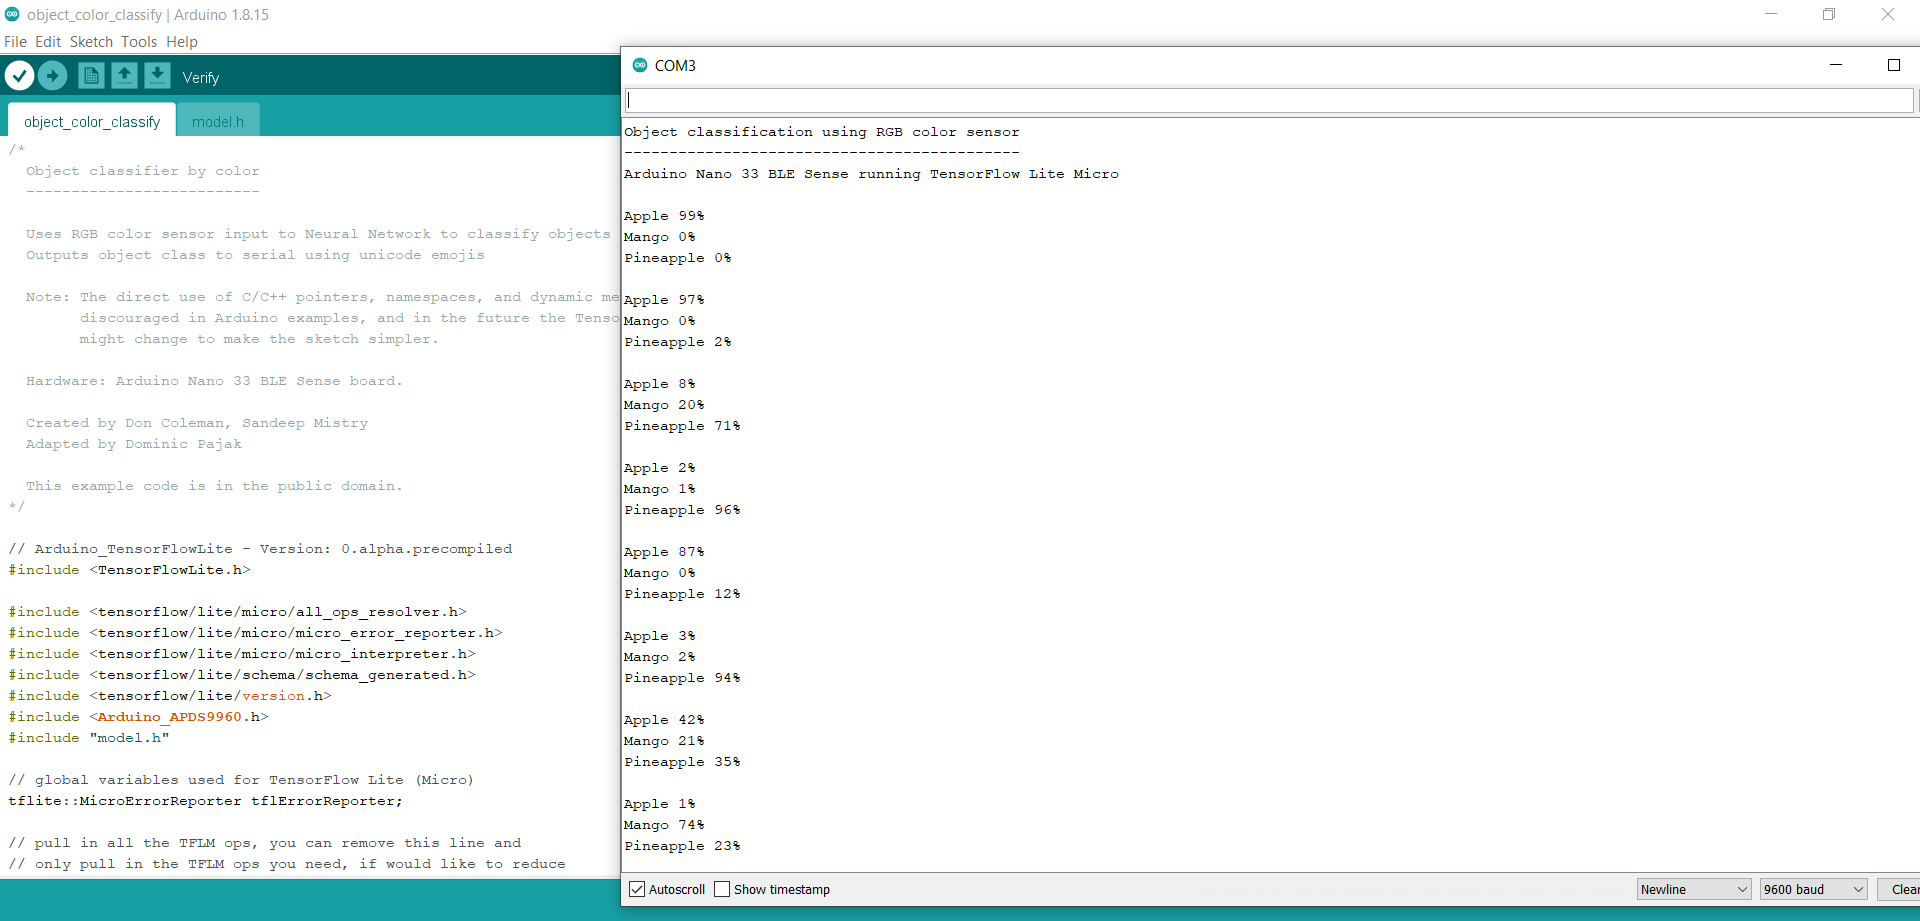
\includegraphics[width=8cm]{Arduino/ArdiunoIDE2/OutputWindow}
    \caption{\textbf{Output Window.}}
    \label{fig:Output Window}		
\end{figure} 


\section{example code for IMU on the Arduino Nano 33 BLE Sense.}


\begin{verbatim}
    #include <Arduino_LSM9DS1.h>
    
    void setup() {
        Serial.begin(9600);
        while (!Serial);
        
        if (!IMU.begin()) {
            Serial.println("Failed to initialize IMU!");
            while (1);
        }
        
        Serial.print("Accelerometer sample rate = ");
        Serial.print(IMU.accelerationSampleRate());
        Serial.println(" Hz");
    }
    
    void loop() {
        float x, y, z;
        
        if (IMU.accelerationAvailable()) {
            IMU.readAcceleration(x, y, z);
            Serial.print("Acceleration X: ");
            Serial.print(x);
            Serial.print(" Y: ");
            Serial.print(y);
            Serial.print(" Z: ");
            Serial.println(z);
        }
    }
\end{verbatim}

This code snippet utilizes the Adafruit CircuitPython library for interacting with the accelerometer sensor on the Arduino Nano 33 BLE Sense. It continuously scans for BLE devices advertising the Adafruit accelerometer service, connects to the first one found, and then reads and prints accelerometer data in the main loop. Make sure to install the required CircuitPython libraries and dependencies before running this code on your Arduino Nano 33 BLE Sense.\cite{Harris:2023}


\section{example code for sensor calibration on the Arduino Nano 33 BLE Sense.}

\begin{lstlisting}[language=C++, caption={Sensor Calibration Example Code}, captionpos=b]
    #include <Arduino_LSM9DS1.h> // Include the LSM9DS1 library for sensor calibration
    
    void setup() {
        Serial.begin(9600); // Initialize serial communication
        while (!Serial); // Wait for Serial to be ready
        
        // Initialize the LSM9DS1 sensor
        if (!IMU.begin()) {
            Serial.println("Failed to initialize IMU!");
            while (1); // End program if initialization fails
        }
        
        // Perform sensor calibration
        Serial.println("Starting sensor calibration...");
        if (!IMU.calibrate()) {
            Serial.println("Calibration failed!");
            while (1); // End program if calibration fails
        }
        Serial.println("Calibration successful!");
    }
    
    void loop() {
        // Your main program loop goes here
    }
\end{lstlisting}

You can add additional code to the loop() function to perform other tasks once sensor calibration is complete.\cite{Rehder:2017}



	\section{Development Environment}

The development environment for the Magic Wand project with Arduino Nano 33 BLE Sense encompasses a combination of hardware and software components tailored to facilitate the implementation of gesture recognition and other functionalities. This environment enables seamless integration between the Arduino Nano 33 BLE Sense board, machine learning algorithms, and communication protocols necessary for project execution. \cite{ArduinoNanoGetStarted:2024}

\subsection*{Hardware Components}

\begin{enumerate}[label=\arabic*.]
    \item \textbf{Arduino Nano 33 BLE Sense}: The core component of the project, featuring integrated BLE connectivity, motion sensors, environmental sensors, and a powerful microcontroller unit.
\end{enumerate}

\subsection*{Software Components}

\begin{enumerate}[label=\arabic*.]
    \item \textbf{Arduino IDE}: The Arduino Integrated Development Environment (IDE) serves as the primary software platform for programming the Arduino Nano 33 BLE Sense board. It provides a user-friendly interface for writing, compiling, and uploading code to the board.
    
    \item \textbf{ArduinoBLE Library}: This library facilitates Bluetooth Low Energy (BLE) communication and interaction with the Arduino Nano 33 BLE Sense board. It enables seamless integration of BLE functionalities into the project code.
    
    \item \textbf{Machine Learning Frameworks}:
    \begin{itemize}
        \item \textbf{TensorFlow}: A popular open-source machine learning framework used for developing and training neural network models. TensorFlow provides robust support for deep learning algorithms and is utilized for gesture recognition tasks in the project.
        \item \textbf{Keras}: Built on top of TensorFlow, Keras offers a high-level neural networks API, enabling rapid prototyping and experimentation with deep learning models. It provides a user-friendly interface for designing and training neural networks, making it ideal for integrating machine learning capabilities into the project.
    \end{itemize}
    
    \item \textbf{Python}: As the primary programming language for machine learning tasks, Python is used extensively within the project environment. It facilitates interaction with TensorFlow, Keras, and other libraries, allowing for seamless development and deployment of machine learning models.
    
    \item \textbf{Operating System}: The project development environment may be hosted on various operating systems, including Windows, macOS, or Linux distributions such as Ubuntu. Each operating system provides essential tools and utilities for software development and board communication.
\end{enumerate}

By leveraging these hardware and software components within the development environment, the Magic Wand project aims to empower users to interact intuitively with the Arduino Nano 33 BLE Sense board through gesture recognition, opening avenues for diverse applications in IoT, robotics, and human-computer interaction.\cite{Kurniawan:2021}


\section{Versions}

\begin{enumerate}
    \item \textbf{Arduino IDE Version}: Specify the version of the Arduino IDE you are using. For example, Arduino IDE 1.8.19.
    
    \item \textbf{ArduinoBLE Library Version}: Mention the version of the ArduinoBLE library you have installed. For instance, ArduinoBLE library version 1.2.0.
    
    \item \textbf{TensorFlow Version}: If you're incorporating machine learning models for gesture recognition, specify the version of TensorFlow. For example, TensorFlow 2.7.0.\cite{ArduinoSoftware:2024}
    
    \item \textbf{Keras Version}: Since you're using Keras for machine learning tasks, mention the version of Keras installed. For instance, Keras 2.8.0.
    
    \item \textbf{Python Version}: Specify the version of Python installed on your system. For example, Python 3.10.0.\cite{PythonDownload:2024}
    
    \item \textbf{Operating System}: Mention the operating system of your development environment, such as Windows 10, macOS Big Sur, or Ubuntu 20.04.
    
    \item \textbf{Any other relevant library versions}: additional libraries like NumPy, SciPy, etc., mention their versions as well.
\end{enumerate}

Providing detailed version information ensures reproducibility and compatibility for your project, allowing others to replicate your development environment accurately.


\section{Description}

It is an open source official Arduino software which used for editing, uploading and
compiling codes in to the Arduino module. It is a cross-platform software which is
available for Operating Systems like Windows, Linux, macOS. It runs on Java platform
and supports a range of Arduino modules. It supports C and C++ languages. The
microcontrollers present on the Arduino boards are programmed which accepts the
information in the form of code. The program written in the IDE is called a sketch
which will generate a Hex file which is then transferred and uploaded in the controller.
The IDE environment is made up of two parts: an editor and a compiler. The editor
is used to write the required code, while the compiler is used to compile and upload
the code to the Arduino Module.\cite{Fezari:2018}
The Menu bar has options such as File in which there are many options including
Opening a new file or existing, Examples-in which we can find sketches for different
applications like Blink, Fade etc. There is an error console at the bottom of the screen
for displaying errors.

The 6 buttons are present on top of the screen are as follows:

\begin{figure}[H]\centering
    
\includegraphics[width=8cm]{MagicWand/ArduinoIDE/ArduinoIcons}
    \caption{\textbf{Menu button.}}
    \label{fig::ArduinoIDEmenubar}		
\end{figure}


\begin{itemize}
    \item	The check mark is used to verify your code. Click this once you have written your code.
    \item	The arrow uploads your code to the Arduino to run.
    \item	The dotted paper will create a new file.
    \item	The upward arrow is used to open an existing Arduino project.
    \item	The downward arrow is used to save the current file.
    \item	The far right button is a serial monitor, which is useful for sending data from the Arduino to the PC for debugging purposes.
    
\end{itemize}
\section{Installation}

To install the Arduino IDE, we need to download the latest version from the Arduino webpage \url{https://www.arduino.cc/en/software}. We can select the version based on the operating system we are using. Here we are installing Arduino 1.8.15 for a Windows 10 operating system. 
The set up file name is arduino-1.8.15-windows.exe and the size of it is 1,17,470 KB. we can specify the path according to our needs. Here the path is set as  \SHELL{C:/Program Files (x86)/Arduino}.

\begin{figure}[H]\centering
    \includegraphics[width=8cm]{MagicWand/ArduinoIDE/MenuBarOptions}
    \caption{\textbf{Menu bar options.}}
    \label{fig::Menu bar options}		
\end{figure}

After the download is done, open the setup file and proceed to install.
Select all the components in the dialog box and click Next.\\

\begin{figure}[H]\centering
    \includegraphics[width=8cm]{MagicWand/ArduinoIDE/ArduinoSetupInstallationOptions}
    \caption{\textbf{Arduino Setup Installation options.}}
    \label{fig:Arduino Setup Installation options}		
\end{figure}

Select the destination folder and click Install

\begin{figure}[H]\centering
    \includegraphics[width=8cm]{MagicWand/ArduinoIDE/ArduinoSetupInstallationFolder}
    \caption{Arduino Setup Installation Folder.}
    \label{fig:Arduino Setup Installation Folder}		
\end{figure}

Once the installation is done, open the Arduino IDE and a default sketch appears on the screen as shows.

\begin{figure}[H]\centering
    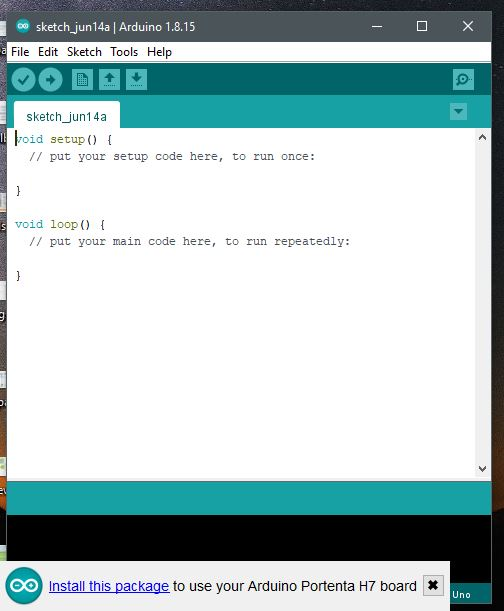
\includegraphics[width=8cm]{MagicWand/ArduinoIDE/ArduinoSketch}
    \caption{Arduino Sketch.}
    \label{fig:Arduino Sketch}		
\end{figure}


It can be seen from the above figure that the basic arduino sketch has two parts. The first part is the function \PYTHON{void setup()} which returns void and we do the intiliaztion such as the output LED color, specifying the core etc. The second part is the function \PYTHON{void loop()} where we define functions which are to be performed through out the loop. These codes are placed between paranthesis \PYTHON{$\{ \}$} and each function has a return type, here it has void return type.

\subsection{Arduino IDE on PC}

Arduino Nano 33 BLE Sense uses the Arduino software integrated development environment (IDE) for programming, which is the most widely used and common (IDE) for all arduino boards that can be run online and offline. This is a open-source Arduino Software (IDE) makes it easy to write code and upload it to the board. There are various version of software which is supported for each operating system (OS) e.g: mac, linux, and windows. Arduino community also provide us to start coding online and save our sketches in the cloud, this online arduino editor is most up-to-date version of the IDE includes all libraries and also supports new Arduino boards. For getting access to these software packages go to the following link \url{https://www.arduino.cc/en/software}  and get more up to date inforamtion, because every single day there are some updates occurs which is available on the link mention above. These software can be used with any Arduino board, the most recent offline arduino IDE 1.8.15 can be seen in Figure,\ref{fig:Arduino Creat Agent Installation}. it is also supportive for all operating systems.


\begin{figure}[H]\centering
    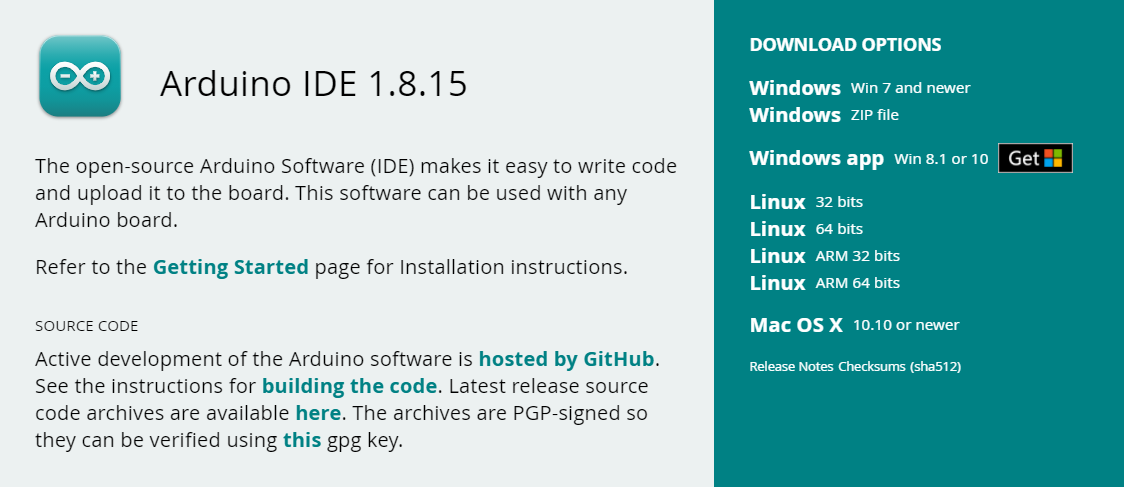
\includegraphics[width=8cm]{MagicWand/ArduinoIDE/ArduinoCreateAgentInstallation}
    \caption{Arduino Create Agent Installation.}
    \label{fig:Arduino Creat Agent Installation}		
\end{figure}

\section{Configuration}

\subsection{Configuration for the Arduino Nano 33 BLE Sense}

To program the Arduino Nano 33 BLE Sense in offline state, we need to install one
of the latest arduino IDE on our desktop. After installation, for getting access to
the Arduino nano 33 ble sense board, we need to make configuration in our IDE. By
opening the IDE, go to tool which can be seen on the uper left corner in IDE, in the
tool there is an option for managed board. At this point we need to write our board
name in the search which is Arduino Nano 33 BLE Sense as shown in figure,Select
the Arduino Mbed OS Boards and install it. The Mbed OS nano board supports also
other nano family boards including Arduino nano 33 ble sense, after installing simply
connect the Arduino Nano 33 BLE Sense to the computer via USB cable.


\begin{figure}[H]\centering
    \includegraphics[width=8cm]{MagicWand/ArduinoIDE/ArduinoMbedOSNanoBoardsInstallation}
    \caption{\textbf{Arduino Mbed OS Nano Boards Installation.}}
    \label{fig:Arduino Mbed OS Nano Boards Installation}		
\end{figure}


\section{First Steps}

\begin{enumerate}
    \item \textbf{Install Arduino IDE}: Begin by installing the Arduino Integrated Development Environment (IDE) on your computer. You can download the IDE from the official Arduino website \href{https://www.arduino.cc/en/software}{download} and follow the installation instructions for your operating system.\cite{Fezari:2018}
    
    \item \textbf{Connect Arduino Nano 33 BLE Sense}: Use a USB cable to connect your Arduino Nano 33 BLE Sense board to your computer.
    
    \item \textbf{Open Arduino IDE}: Launch the Arduino IDE application on your computer.
    
    \item \textbf{Select Board}: In the Arduino IDE, navigate to the menu ``Tools'' and select ``Board''. Choose ``Arduino Nano 33 BLE'' from the list of available boards.
    
    \item \textbf{Select Port}: Still in the menu ``Tools'', go to the ``Port'' option and select the port to which your Arduino Nano 33 BLE Sense board is connected. On Windows, it will typically be something like "COMX", and on macOS, it will be "/dev/cu.usbmodemXXXX".
    
    \item \textbf{Verify Connection}: Once the board and port are selected, verify that your Arduino Nano 33 BLE Sense board is successfully connected to the Arduino IDE. You can do this by checking the bottom right corner of the IDE window for a message indicating the board and port.
    
    \item \textbf{Open Example Sketch}: To ensure that your setup is working correctly, you can open a built-in example sketch. Go to the "File" menu, select "Examples", then navigate to "01.Basics" and choose the "Blink" example. This sketch will blink the built-in LED on the Arduino Nano 33 BLE Sense board.
    
    \item \textbf{Upload Example Sketch}: Click on the "Upload" button (right arrow icon) in the Arduino IDE toolbar to compile and upload the example sketch to your Arduino Nano 33 BLE Sense board. You should see the built-in LED blinking once the upload is complete.
    
    \item \textbf{Verify Operation}: Verify that the LED on your Arduino Nano 33 BLE Sense board is blinking. This confirms that your development environment is set up correctly and your board is communicating with the Arduino IDE.
    
    \item \textbf{Explore Further}: Now that you have successfully completed the initial setup and verification steps, you can explore more advanced features and functionalities of the Arduino Nano 33 BLE Sense board and the Arduino IDE. Consider experimenting with different example sketches, sensors, and communication protocols to familiarize yourself with the capabilities of your board.\cite{ArduinoIntroduction:2018}
\end{enumerate}

Congratulations! You have completed the first steps in setting up the development environment for your Magic Wand project with Arduino Nano 33 BLE Sense. You're now ready to proceed with implementing your project's functionality and features.

\section{Program "Hello World"}

\begin{enumerate}
    \item \textbf{Setup Arduino IDE}: Make sure you have the Arduino IDE installed on your development machine. You can download it from the official Arduino website and follow the installation instructions for your operating system.
    
    \item \textbf{Connect Arduino Nano 33 BLE Sense}: Connect your Arduino Nano 33 BLE Sense board to your computer using a USB cable.\cite{Fezari:2018}
    
    \item \textbf{Open Arduino IDE}: Launch the Arduino IDE on your computer.
    
    \item \textbf{Select Board}: Go to the "Tools" menu, then select "Board", and choose "Arduino Nano 33 BLE" from the list of available boards.
    
    \item \textbf{Select Port}: In the "Tools" menu, select the port to which your Arduino Nano 33 BLE Sense is connected. It will typically appear as something like "COMX" on Windows or "/dev/cu.usbmodemXXXX" on macOS.
    
    \item \textbf{Open New Sketch}: Click on "File" > "New" to open a new sketch.
    
    \item \textbf{Write Code}: In the new sketch window, write the following code:
    
    \begin{verbatim}
        void setup() {
            // Initialize serial communication
            Serial.begin(9600);
            
            // Wait for serial monitor to open
            while (!Serial);
            
            // Print "Hello, World!" to serial monitor
            Serial.println("Hello, World!");
        }
        
        void loop() {
            // Empty loop
        }
    \end{verbatim}
    
    \item \textbf{Upload Code}: Click on the "Upload" button (right arrow icon) to compile and upload the code to your Arduino Nano 33 BLE Sense board.
    
    \item \textbf{View Output}: Once the upload is complete, open the Serial Monitor by clicking on "Tools" > "Serial Monitor" (or press Ctrl+Shift+M). You should see "Hello, World!" printed in the Serial Monitor at a baud rate of 9600.
    
    \item \textbf{Verify Operation}: Verify that "Hello, World!" is successfully printed in the Serial Monitor. This confirms that your Arduino Nano 33 BLE Sense board is properly set up and functioning.
\end{enumerate}

programmed a "Hello, World!" example for your Magic Wand project using Arduino Nano 33 BLE Sense. This serves as a basic test to ensure that your development environment is configured correctly and your hardware is working as expected.


\subsection{Description of Basic Sketch for Printing 'Hello'}

To test the development environment and the basic functionality of the hardware, a simple example sketch that controls only one LED is suitable. This sketch provides the Arduino \ac{ide}. Under the path \FILE{File/Examples/01.Basics}, small example sketches can be selected. Here, the example \FILE{Fade} is used. In this case, the built-in LED, which is an RGB LED, is utilized. 


\begin{lstlisting}
    int brightness = 0;  // how bright the LED is
    int fadeAmount = 5;  // how many points to fade the LED by
    
    // the setup routine runs once when you press reset:
    void setup() {
        // declare LED_BUILTIN to be an output:
        pinMode(LED_BUILTIN, OUTPUT);
    }
    
    // the loop routine runs over and over again forever:
    void loop() {
        // set the brightness of LED_BUILTIN:
        analogWrite(LED_BUILTIN, brightness);
        
        // change the brightness for next time through 
        //the loop:
        brightness = brightness + fadeAmount;
        
        // reverse the direction of the fading at the ends 
        //of the fade:
        if (brightness <= 0 || brightness >= 255) {
            fadeAmount = -fadeAmount;
        }
        // wait for 30 milliseconds to see the dimming 
        //effect
        delay(30);
    }
\end{lstlisting}


As a result, the brightness of the built-in LED should gradually fade in and out.

